\documentclass[11pt,a4paper]{article}
\usepackage[a4paper,margin=2.5cm,headheight=14pt]{geometry}
\usepackage{mathptmx}              % Times text and maths
\usepackage[T1]{fontenc}
\usepackage{amsmath,amssymb}
\usepackage{graphicx,xcolor}
\usepackage{booktabs,tabularx,multirow}
\usepackage{algorithm}
\usepackage[noend]{algpseudocode}
\usepackage[font=small,labelfont=bf]{caption}
\usepackage{subcaption}
\usepackage{enumitem}
\usepackage{microtype}
\usepackage{fancyhdr}
\usepackage{titlesec}
\usepackage[hidelinks]{hyperref}
\usepackage{xurl}
\usepackage{tikz}
\usetikzlibrary{positioning,arrows.meta}

\definecolor{coverblue}{HTML}{4F81BD}
\setlist{itemsep=1pt,topsep=3pt,parsep=0pt}
\setlength{\parskip}{4pt}
\linespread{1.07}
\titleformat{\section}{\large\bfseries}{\thesection}{0.6em}{}
\titleformat{\subsection}{\normalsize\bfseries}{\thesubsection}{0.6em}{}
\titlespacing*{\section}{0pt}{10pt}{4pt}
\titlespacing*{\subsection}{0pt}{7pt}{3pt}
\setlength{\textfloatsep}{9pt plus 2pt minus 2pt}
\setlength{\floatsep}{8pt plus 2pt minus 2pt}
\setlength{\intextsep}{8pt plus 2pt minus 2pt}
\captionsetup{skip=4pt}
\renewcommand{\algorithmicrequire}{\textbf{Input:}}
\renewcommand{\algorithmicensure}{\textbf{Output:}}

\pagestyle{fancy}
\fancyhf{}
\fancyhead[L]{\small Lightpath: Latency-Aware Cloud Task Placement}
\fancyhead[R]{\small Design and Analysis of Algorithms}
\fancyfoot[C]{\small\thepage}
\renewcommand{\headrulewidth}{0.4pt}

\newcommand{\R}{\mathbb{R}}
\newtheorem{lemma}{Lemma}
\newenvironment{proofsketch}{\par\noindent\textit{Proof sketch.}\ }{\hfill$\square$\par}

\begin{document}
% Cover page (matches the department's report style)
\begin{titlepage}
  \centering
  \vspace*{0.6cm}
  {\fontsize{19}{28}\selectfont\bfseries DESIGN AND ANALYSIS OF ALGORITHMS\par}
  \vspace{0.25cm}
  {\fontsize{13}{18}\selectfont Project Report\par}
  \vspace{0.7cm}
  {\fontsize{17}{25}\selectfont\bfseries Lightpath: Latency-Aware Cloud Task Placement\\ on Network Graphs\par}
  \vspace{0.35cm}
  {\fontsize{13}{19}\selectfont Graph Algorithms, Dynamic Programming and Greedy Scheduling\\ for Replica and VM Placement\par}
  \vfill
  
\includegraphics[width=0.56\textwidth]{figures/woxsen_logo.png}\par
  \vfill
  {\fontsize{15}{20}\selectfont\color{coverblue} Team Members\par}
  \vspace{0.45cm}
  {\fontsize{13}{18}\selectfont Naman Singla -- 25WU0101084\par}
  \vspace{0.3cm}
  {\fontsize{13}{18}\selectfont Mohak Gupta -- 25WU0101074\par}
  \vspace{0.55cm}
  {\fontsize{15}{20}\selectfont\color{coverblue} Faculty\par}
  \vspace{0.45cm}
  {\fontsize{13}{18}\selectfont Dr. Monday Jubrin Abdullahi\par}
  \vspace{0.55cm}
  {\fontsize{13}{18}\selectfont{\color{coverblue}\fontsize{15}{20}\selectfont Section}\,:\, CSE RHINOS\par}
  \vspace{0.3cm}
  {\fontsize{13}{18}\selectfont{\color{coverblue}\fontsize{15}{20}\selectfont Academic Year}\,:\, 2026--2027\par}
  \vspace*{0.8cm}
\end{titlepage}

\setcounter{page}{1}
%======================================================================
\section{Introduction and Problem Statement}\label{sec:intro}

\subsection{Course context}
This report documents \emph{Lightpath}, our project for the Design and Analysis of Algorithms (DAA) course at Woxsen University. Of the problem statements offered in the brief, we chose \textbf{Cloud Task Placement}: servers are nodes, link latencies are edge weights, and replicas or virtual machines (VMs) must be placed to minimise average latency while respecting server capacity. The brief asks for minimum spanning trees for the backbone, shortest paths for routing and dynamic programming for placement selection, together with greedy schedulers, experiments that vary size, density and capacity, and policy outputs. Lightpath implements every item on that list and adds an exact optimiser so that the quality of each heuristic can be measured rather than assumed.

\subsection{Motivation: why placement is a real algorithmic problem}
A request to an online service, whether a video stream, a payment or a search, travels from the user's nearest network site to a server that holds a copy of the service. The delay the user feels is dominated by the distance the signal travels through fibre and the number of switches it crosses. Putting copies close to users makes them fast, but three concerns pull against each other:
\begin{itemize}[leftmargin=*]
  \item \textbf{Latency.} Every user should reach a nearby copy. This pushes copies towards the cities with the most demand.
  \item \textbf{Capacity.} Each server has limited CPU and memory. A popular city cannot host every service, and a server used by one service may be needed by another.
  \item \textbf{Cost.} Every copy costs money per hour, and every server that is switched on has a running cost. The budget limits how many copies we can buy.
\end{itemize}
Deciding \emph{where to run what} under these pressures is a combinatorial optimisation problem on a graph. It touches almost every family of algorithms in the course: shortest paths to measure distance, spanning trees to design the network, dynamic programming to spend a budget, and greedy methods to make fast decisions when exact search is too slow.

\subsection{What makes it hard}
If there were only one service, no capacity limits and a fixed number of copies, the problem would be exactly the classical \emph{p-median} problem: choose $p$ sites so that the total distance from every client to its nearest chosen site is as small as possible. The p-median problem is NP-hard on general graphs \cite{kariv1979}, and adding capacities adds bin-packing structure, which is NP-hard by itself. No known algorithm solves every instance exactly in polynomial time. Our approach therefore uses exact algorithms wherever a sub-problem is tractable, fast greedy heuristics for the hard placement step, and an exact solver on smaller networks to measure how far the heuristics are from the true optimum.

\subsection{Objectives and contributions}
The project set out to answer three questions:
\begin{enumerate}[label=\textbf{Q\arabic*},leftmargin=*]
  \item Which classical algorithm is the right one for each stage, and do their theoretical bounds match what we measure?
  \item How close do fast greedy schedulers get to the true optimum, and what does closing the gap cost?
  \item How do network size, density, server capacity and budget change the answer?
\end{enumerate}
Our contributions are: a seven-stage pipeline that solves capacitated, budgeted, multi-service placement; implementations of every algorithm from first principles (including four priority queues and union-find); a transfer-cost model with negative edges that motivates Bellman-Ford and Johnson; ten test networks including India, Nigeria and the Woxsen campus; eight experiments with an exact reference; 191 automated tests; and an interactive website that explains and demonstrates all of it.

%======================================================================
\section{Problem Formulation}\label{sec:model}

\subsection{Inputs}
The cloud is modelled as a weighted, undirected graph $G=(V,E)$:
\begin{itemize}[leftmargin=*]
  \item \textbf{Nodes} $V$ are network sites. Most are servers with a CPU capacity (vCPU), a memory capacity (GB) and an hourly running cost. Some are routers that forward traffic but cannot host anything.
  \item \textbf{Edges} $E$ are fibre links. Each link carries a \textbf{latency} in milliseconds and a bandwidth. For networks with real coordinates, latency is computed from distance: light in fibre covers about 200\,km per millisecond, cables are about 30\,\% longer than the straight line, and each hop adds about 0.3\,ms of switching.
  \item \textbf{Services} are the workloads, such as web front end, video transcoding or payments. Each needs a fixed amount of CPU and memory per copy, costs a fixed amount per copy-hour, has a priority, a minimum and maximum number of copies, and a \textbf{demand}: how many requests per second each city sends to it.
  \item \textbf{Budgets} limit the total hourly spend on copies and, optionally, on switching servers on.
\end{itemize}
Storage is an adjacency list, so memory grows with the number of nodes plus links rather than with the square of the number of nodes. Real networks are sparse, with each city linked to only a few others, so this matters.

\subsection{Objective}
Every user is served by the nearest copy of the service they request, measured along the shortest path in the network. The quantity we minimise is the \textbf{demand-weighted average latency}:
\[
\text{average latency} \;=\; \frac{\sum\ (\text{requests from city } c \text{ for service } j)\times(\text{distance from } c \text{ to the nearest copy of } j)}{\text{total requests}}.
\]
Requests from higher-priority services count more. We also report the 95th-percentile and worst-case latency, because an average can hide a few badly served cities.

\subsection{Constraints}
A plan is valid only if:
\begin{itemize}[leftmargin=*]
  \item every service has between its minimum and maximum number of copies, and at most one copy per server (so one server failure cannot take out two copies);
  \item on every server, the CPU and memory used by the copies it hosts do not exceed its capacity;
  \item the total hourly cost of all copies stays within the VM budget, and if a server budget is set, only servers bought within it are used.
\end{itemize}

\subsection{Transfer costs and negative edges}
Copies of the same service must synchronise data. Moving a gigabyte from site $u$ to site $v$ costs a small base fee plus a per-millisecond charge, adjusted by the difference in regional price levels between $u$ and $v$. Core data centres are cheaper than edge sites, so sending data towards a more expensive region earns a \emph{rebate}. Some arcs therefore have a \textbf{negative cost}: in the India network, 24 of 88 directed arcs are negative.

Negative edges break Dijkstra's algorithm, which is why the brief's Bellman-Ford and Johnson algorithms have a genuine role here. Negative edges are only dangerous if they form a \emph{negative cycle}, because then the cost could be lowered for ever by going round the loop. Our cost model rules this out (Lemma~\ref{lem:nocycle}, Section~\ref{sec:proofs}).

\subsection{Infeasibility handling}
The system reports problems instead of crashing or silently returning a wrong plan:
\begin{itemize}[leftmargin=*]
  \item \textbf{Invalid network.} Before solving, the instance is validated: links must have positive latency, services must have valid replica ranges, and every demand must come from a real site. Disconnected networks are flagged, and the spanning tree becomes a spanning forest.
  \item \textbf{Not enough capacity.} If the minimum copies cannot all fit, the sizing stage reports it, and strategies that cannot place every copy are marked \emph{infeasible} with the reason. They are never shown as valid plans.
  \item \textbf{A service no server can host.} Such a service is kept at zero copies and the same penalty is applied in both the heuristics and the exact solver, so their scores remain comparable.
\end{itemize}

%======================================================================
\section{Technology Stack and Justification}\label{sec:tech}
Lightpath has three layers: a Python engine that contains every algorithm, a small web API, and a browser dashboard. Table~\ref{tab:tech} gives each tool and the reason it was chosen.

\begin{table}[!htbp]
\centering\small
\caption{Technology stack and the rationale for each choice.}\label{tab:tech}
\begin{tabularx}{\textwidth}{@{}p{2.9cm}p{4.2cm}X@{}}
\toprule
Tool & Role in the project & Why it was chosen\\
\midrule
Python 3 (\texttt{cloudplace} package) & All algorithms, the problem model, data generators, the solver and the experiments & Readable enough that every algorithm can be written from first principles and checked line by line against the textbook. Graphs, heaps, union-find, the DPs and the greedy methods are our own code, not library calls. \\
NumPy & Vectorised Floyd--Warshall and the distance matrices & One vectorised version of Floyd--Warshall runs the same $\Theta(n^3)$ algorithm much faster than pure Python. That made Experiment E2 possible, comparing constant factors with asymptotics. \\
SciPy (HiGHS solver) & Exact MILP used only as a referee & An independent, proven-optimal answer is the only honest way to measure a heuristic's gap. It checks our algorithms and is never used to produce them. \\
FastAPI + Uvicorn & REST API serving datasets, solving and step-by-step traces & Typed request models catch bad input early, and one process serves both the API and the website. \\
React 18 + TypeScript + Vite & Interactive dashboard & State-driven rendering suits an app where one change (network, budget, start city) must update the map, tables and charts together. TypeScript catches data-shape errors between engine and UI. \\
Custom SVG map & Network drawing, routes, step animations & Full control over highlighting exactly the edge or node each algorithm touches at each step, without a heavy graph library. \\
pytest, Hypothesis, NetworkX & 191 automated tests & NetworkX is an independent reference for every graph algorithm; Hypothesis generates random inputs for heap tests. \\
\bottomrule
\end{tabularx}
\end{table}

\noindent\textbf{Why a working application and not only a script.} The brief asks for a dashboard and policy outputs. An interactive site also makes the algorithms visible: in the Algorithm Lab a viewer can watch Dijkstra settle cities one by one, or see Bellman-Ford handle a rebate link that would fool Dijkstra. Running on saved results, the site also works offline, so it can be demonstrated without installing Python.

%======================================================================
\section{Algorithms Used, and Why Each One Was Chosen}\label{sec:algo}
This section is the analytical core of the report. For each stage it states what the stage must achieve, which algorithm was selected, why that algorithm fits, and which alternatives were set aside. Fig.~\ref{fig:pipeline} shows how the stages connect: each one answers one question, and its output feeds the next.

\begin{figure}[!htbp]
\centering
\resizebox{\textwidth}{!}{%
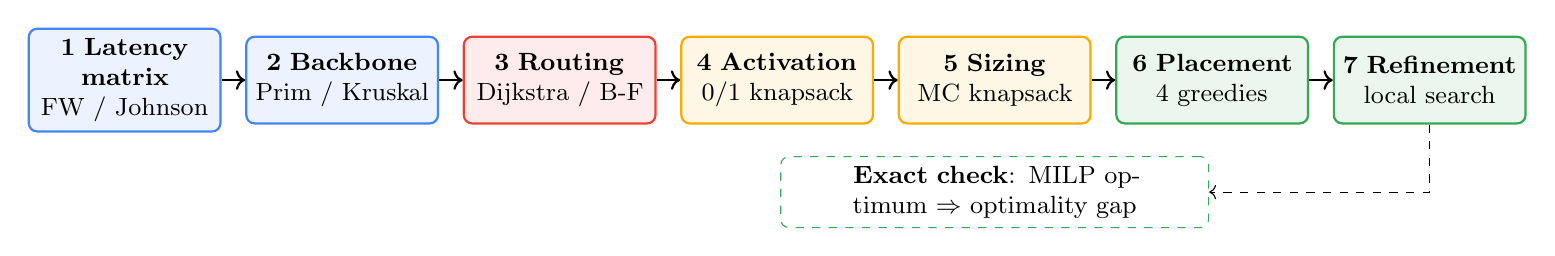
\begin{tikzpicture}[font=\small,node distance=3mm,
  st/.style={draw=#1,fill=#1!10,rounded corners=3pt,minimum height=11mm,text width=22mm,align=center,line width=0.8pt}]
  \definecolor{gb}{HTML}{4285F4}\definecolor{gr}{HTML}{EA4335}\definecolor{gy}{HTML}{F9AB00}\definecolor{gg}{HTML}{34A853}
  \node[st=gb] (a) {\textbf{1 Latency matrix}\\FW / Johnson};
  \node[st=gb,right=of a] (b) {\textbf{2 Backbone}\\Prim / Kruskal};
  \node[st=gr,right=of b] (c) {\textbf{3 Routing}\\Dijkstra / B-F};
  \node[st=gy,right=of c] (d) {\textbf{4 Activation}\\0/1 knapsack};
  \node[st=gy,right=of d] (e) {\textbf{5 Sizing}\\MC knapsack};
  \node[st=gg,right=of e] (f) {\textbf{6 Placement}\\4 greedies};
  \node[st=gg,right=of f] (g) {\textbf{7 Refinement}\\local search};
  \foreach \x/\y in {a/b,b/c,c/d,d/e,e/f,f/g} \draw[->,thick] (\x) -- (\y);
  \node[draw=gg,dashed,rounded corners=3pt,below=4mm of e,text width=52mm,align=center,minimum height=8mm] (x) {\textbf{Exact check}: MILP optimum $\Rightarrow$ optimality gap};
  \draw[->,dashed] (g.south) |- (x.east);
\end{tikzpicture}}
\caption{The Lightpath pipeline. Stages 1--3 are exact polynomial algorithms, 4--5 exact dynamic programs, and 6--7 fast heuristics whose distance from the optimum is measured by the exact MILP.}\label{fig:pipeline}
\end{figure}

\subsection{Supporting data structures}
\subsubsection{Adjacency list}
Each site keeps a list of its neighbours with the link's latency, bandwidth and cost. Memory is proportional to sites plus links, and visiting a site's neighbours costs only its number of links. An adjacency matrix was rejected: it wastes $n^2$ cells on links that do not exist and makes every neighbour scan cost $n$.

\subsubsection{Four priority queues}
Dijkstra and Prim repeatedly need the closest unfinished site, which is a priority-queue job. We implemented four queues behind one interface (\emph{push}, \emph{pop-minimum}, \emph{decrease-key}) so the same algorithm can run on any of them:
\begin{itemize}[leftmargin=*]
  \item \textbf{Binary heap} with a position map: every operation in $O(\log n)$.
  \item \textbf{Fibonacci heap} \cite{fredman1987}: insert and decrease-key in amortised $O(1)$, extract-min in $O(\log n)$. It is the textbook way to get the best bound for Dijkstra and Prim.
  \item \textbf{Pairing heap}: simpler than Fibonacci with good practical speed.
  \item \textbf{Lazy heap} (Python's built-in \texttt{heapq}): instead of decreasing a key, it pushes a new entry and skips stale ones when they surface.
\end{itemize}
Implementing all four was a deliberate choice: Experiment E1 tests whether the heap with the best Big-O is also the fastest in practice. It is not.

\subsubsection{Union-find}
Kruskal must check quickly whether a link would close a loop. Union-find with \emph{union by rank} and \emph{path compression} does this in almost constant amortised time, $O(\alpha(n))$ per operation \cite{tarjan1975}.

\subsection{Minimum spanning tree: Prim's and Kruskal's algorithms}
\subsubsection{Why an MST at all?}
Every physical link costs money to build and maintain. The cheapest way to connect every site with no redundant link is the \textbf{minimum spanning tree}: a set of $n-1$ links that connects all sites with the smallest total latency. In Lightpath the MST is the \emph{provisioning backbone}, the first set of links an operator would build. It is also used to measure \emph{stretch}: how much slower requests would be if they could only travel along the backbone.

\subsubsection{Why implement both Prim and Kruskal}
Both find the same cheapest tree but in different ways, and each wins in a different situation.
\begin{itemize}[leftmargin=*]
  \item \textbf{Prim} \cite{prim1957} grows a single tree from a start city, always adding the cheapest link that reaches a new city. Using our heaps it runs in $O(E\log V)$, or $O(E+V\log V)$ with a Fibonacci heap. It never sorts the whole edge list, which makes it better on \emph{dense} graphs.
  \item \textbf{Kruskal} \cite{kruskal1956} sorts all links from cheapest to most expensive and keeps each one unless union-find reports that it would close a loop. Its cost is dominated by the sort, $O(E\log E)$, which is small on \emph{sparse} graphs.
\end{itemize}
The pipeline chooses automatically: \textbf{Prim if $E > V\log_2 V$, otherwise Kruskal}. Experiment E3 confirms the rule. On sparse graphs Kruskal took 1.5\,ms against Prim's 3.7\,ms; on dense graphs Prim took 42\,ms against Kruskal's 126\,ms. Both always returned the same tree weight.

\subsubsection{Alternatives considered}
\textbf{Bor\r{u}vka's algorithm} grows many fragments in parallel. Its advantage is parallelism, which a single-threaded Python program does not use, so we did not implement it. \textbf{Steiner trees} connect only a chosen subset of sites. They do not match our assumption that every site belongs to the backbone.

\subsection{Single-source shortest paths: Dijkstra and Bellman-Ford}
\subsubsection{Role in the pipeline}
Once copies are placed, every request must be \emph{routed}: we need the actual path from each city to its nearest copy, hop by hop, for the route table that operators use. Copies of the same service must also synchronise, and that traffic should take the \emph{cheapest} route in dollars per gigabyte. These are two single-source shortest-path problems with different weights.

\subsubsection{Dijkstra for latency}
Dijkstra's algorithm \cite{dijkstra1959} repeatedly takes the closest unsettled city from a priority queue and declares its distance final, then updates its neighbours. Latency can never be negative, so Dijkstra is correct and fast: $O((V+E)\log V)$ with a binary heap. In the Algorithm Lab it also demonstrates an important property: if only one destination matters, Dijkstra can \emph{stop} as soon as that destination is settled, because its distance can no longer change.

\subsubsection{Bellman-Ford for transfer cost}
For dollars per gigabyte, some links are rebates with negative cost. Dijkstra can then give wrong answers, because a city it has already settled might be reached more cheaply later through a negative link. \textbf{Bellman-Ford} \cite{bellman1958} relaxes every link in rounds. After round $i$, every route that uses at most $i$ links is correct, so $V-1$ rounds are enough. Any improvement in round $V$ would reveal a negative cycle, which our implementation detects and reports. It is slower, $O(VE)$, but it is the right tool when weights can be negative. In Lightpath it computes the cheapest replica-synchronisation routes.

\subsubsection{Why both, and not one}
Using Bellman-Ford everywhere would be correct but needlessly slow for latency, at 490\,ms against 144\,ms at 4000 sites in E1. Using Dijkstra everywhere would be fast but wrong for costs with rebates. Each is used exactly where its guarantee holds.

\subsection{All-pairs shortest paths: Floyd--Warshall and Johnson}
\subsubsection{Role in the pipeline}
Placement must try many candidate servers for every service, and each trial needs the distance from every city to every server. Computing those distances once, as a full \textbf{latency matrix} with an entry for every pair of sites, makes each trial a cheap table lookup. This matrix is the input to every later stage.

\subsubsection{Floyd--Warshall}
Floyd--Warshall \cite{floyd1962} is dynamic programming over intermediate cities. The best route from $i$ to $j$ that may pass through cities $1..k$ either avoids city $k$ or goes through it once, so the table is updated with \(d[i][j] = \min(d[i][j],\ d[i][k] + d[k][j])\) for every $k$. It runs in $\Theta(V^3)$ time and handles negative edges. Its triple loop is also easy to vectorise: our NumPy version runs the same algorithm many times faster than pure Python.

\subsubsection{Johnson}
Johnson's algorithm \cite{johnson1977} targets sparse graphs with negative edges. It runs Bellman-Ford once from an added helper vertex to get a \emph{potential} $h$ for every city, then reweights every link to $w + h(u) - h(v)$, which is never negative. Dijkstra can then run safely from every city. Every route between the same two cities changes by the same amount, so shortest routes stay shortest. The total is $O(VE + V(V+E)\log V)$, better than $V^3$ when the graph is sparse.

\subsubsection{The choice rule, and what the experiment taught us}
The pipeline treats a graph as sparse when $E\log V < V^2$ and then uses repeated Dijkstra (or Johnson if any weight is negative); dense graphs use Floyd--Warshall. Experiment E2 tested this rule. On dense graphs it was clearly right: at 400 sites, NumPy Floyd--Warshall took 277\,ms against Johnson's 5015\,ms. On sparse graphs, Big-O favours Johnson, yet NumPy Floyd--Warshall was still fastest at this size (285\,ms against 985\,ms). The lesson is that \emph{constant factors and implementation matter as much as asymptotics}, so a choice rule should be calibrated by measurement.

\subsection{Dynamic programming: two knapsack problems}
\subsubsection{Why dynamic programming here}
Two budget decisions have exactly the structure of knapsack problems: a set of items with costs and values, a fixed budget, and the goal of the most value within budget. A greedy rule such as ``best value per dollar first'' can be fooled: a cheap item may block a better combination. Dynamic programming considers every budget level systematically and is guaranteed optimal. Budgets are in steps of \$0.01, so the tables stay small enough to be fast.

\subsubsection{0/1 knapsack: which servers to switch on}
When a server budget is set, each server is either on or off. Its \emph{value} is the latency saving it offers and its \emph{weight} is its hourly cost. The DP table \(\mathrm{OPT}[i][w]\) holds the best value using the first $i$ servers with budget $w$: server $i$ is either skipped, keeping \(\mathrm{OPT}[i-1][w]\), or taken, giving its value plus \(\mathrm{OPT}[i-1][w - \text{cost}_i]\). Time and space are $\Theta(nW)$, where $W$ is the budget in cents. Experiment E8 measured about 97\,ns per table cell, growing exactly linearly as predicted.

\subsubsection{Multiple-choice knapsack: how many copies of each service}
Each service must take \emph{exactly one} option from its group: 1 copy, 2 copies, 3 copies and so on, each with a cost and an estimated latency saving. This is the multiple-choice knapsack problem. The DP processes one service at a time and, for every budget level, picks the best option for that service plus the best result for the earlier services with the remaining budget. Because the savings are estimated without capacity limits, a \emph{capacity repair} step then removes the largest extra copies until first-fit-decreasing packing confirms that everything fits. This guarantees that a feasible placement exists before the placement stage starts. Experiment E7 shows the payoff: raising the India budget from \$2.41 to \$7.51 per hour cut average latency from 4.34\,ms to 1.28\,ms.

\subsubsection{Alternatives considered}
Solving the whole placement as one giant DP over every server's remaining capacity would be exact, but its table grows with the \emph{product} of all server capacities. That is impossible for networks of 25 to 150 sites. We therefore use DP where its tables are small (budgets) and greedy methods where they would explode (placement).

\subsection{Greedy schedulers for placement}
\subsubsection{Why greedy}
Choosing the exact server for every copy is the NP-hard heart of the problem. A greedy method makes one good local choice at a time, never undoes it, and finishes in polynomial time. We built four greedy schedulers because each optimises a different concern, and the experiments compare them.
\begin{itemize}[leftmargin=*]
  \item \textbf{Demand-first.} Services with the most traffic choose first, and each copy goes to the free server nearest the next demand hotspot. Simple and intuitive.
  \item \textbf{Marginal gain (CELF).} At every step, add the single copy that reduces total latency the most. Benefits shrink as more copies open (the function is \emph{submodular}), so old estimates can be re-checked lazily instead of recomputed (CELF). Without capacity limits this greedy achieves at least $1-1/e\approx63\,\%$ of the best possible saving \cite{nemhauser1978}.
  \item \textbf{Regret.} Place first the service that would lose the most if it missed its best server, which is the gap between its best and second-best options. This protects services with few good choices from being crowded out.
  \item \textbf{FFD packing.} First-fit decreasing: place the largest copies first, each on a well-located server that fits. It focuses on \emph{fitting} capacity rather than latency; plain FFD uses at most $\tfrac{11}{9}\mathrm{OPT}+\tfrac{6}{9}$ bins.
\end{itemize}

\subsection{Local search refinement}
Greedy methods never revisit a decision, so they can lock in early mistakes. Local search repeatedly tries two kinds of move: \textbf{relocate} (move one copy to a free server) and \textbf{swap} (exchange copies of two services between two servers when both fit). Any move that lowers average latency is kept. Every accepted move strictly improves the plan and there are finitely many plans, so the search always stops. For the uncapacitated version, single-swap local optima are within a factor of 5 of optimal; in practice we observe about 0.5\,\%. Local search is what turns 9--38\,\% greedy gaps into near-optimal plans.

\subsection{The exact referee: a mixed-integer program}
To know whether a heuristic is good, we need the true optimum. On networks small enough, Lightpath formulates placement as a \textbf{mixed-integer linear program} (MILP): binary variables say which server hosts which copy, and the constraints are exactly those of Section~\ref{sec:model}. It is solved with the open-source HiGHS solver \cite{huangfu2018} through SciPy. When the program is too large, we report its linear relaxation as a lower bound instead. The MILP is a \emph{checking tool}: every stage of our own pipeline is implemented by hand, and the MILP only tells us how far each heuristic is from the best possible answer.

\subsection{Batch scheduling}
Background batch jobs, such as nightly analytics, are scheduled with the classic greedy \textbf{LPT} rule: longest job first, each assigned to the server lane where it will finish earliest once its input data arrives over the network. Without transfer delays, LPT is within $\tfrac43$ of the optimal finishing time.

%======================================================================
\section{System Design (UML)}\label{sec:uml}
This section describes Lightpath in standard UML views: who uses the system (use cases), how it is split into deployable parts (components), the main classes and their relationships (class diagram), what happens during one solve request (sequence diagram), and the decision flow of the solver (activity diagram).

\tikzset{
  cls/.style={draw, rectangle split, rectangle split parts=3, rectangle split part fill={blue!12,white,white},
              font=\scriptsize, align=left, inner sep=2pt, text width=#1},
  cls/.default=3.3cm,
  comp/.style={draw, fill=blue!6, rounded corners=1pt, font=\scriptsize, align=center, minimum height=8mm, inner sep=3pt},
  uc/.style={draw, ellipse, fill=yellow!10, font=\scriptsize, align=center, minimum width=26mm, minimum height=7mm, inner sep=1pt},
  act/.style={draw, rounded corners=5pt, fill=green!8, font=\scriptsize, align=center, minimum width=30mm, minimum height=6mm},
  dec/.style={draw, diamond, aspect=2.4, fill=orange!12, font=\scriptsize, align=center, inner sep=1pt},
  inh/.style={-{Triangle[open,length=2.4mm,width=2.4mm]}},
  comp-arr/.style={{Diamond[length=2.6mm,width=1.8mm]}-},
  agg/.style={{Diamond[open,length=2.6mm,width=1.8mm]}-},
  dep/.style={-{Stealth[length=2mm]}, dashed},
  ass/.style={-{Stealth[length=2mm]}},
}

\subsection{Use-case diagram}
Fig.~\ref{fig:usecase} shows the three actors. A \emph{network planner} uses the studio to load or generate networks and obtain placement policies. A \emph{student or instructor} uses the algorithm lab and experiment pages to study the algorithms. A \emph{researcher} runs the experiment suite and exports data. All actions go through the dashboard or the Python API.

\begin{figure}[!htbp]
\centering
\begin{tikzpicture}[font=\scriptsize]
  \pgfdeclarelayer{bg}\pgfsetlayers{bg,main}
  \begin{pgfonlayer}{bg}\draw[rounded corners, thick, fill=gray!3] (-3.7,-3.15) rectangle (3.7,3.15);\end{pgfonlayer}
  \node[anchor=north] at (0,3.1) {\bfseries Lightpath system};
  \node[uc] (u1) at (-1.75, 2.15) {Load / generate\\network};
  \node[uc] (u2) at ( 1.75, 2.15) {Solve placement\\policy};
  \node[uc] (u3) at (-1.75, 0.95) {Compare\\strategies};
  \node[uc] (u4) at ( 1.75, 0.95) {Export routes,\\schedule, data};
  \node[uc] (u5) at (-1.75,-0.35) {Step through an\\algorithm trace};
  \node[uc] (u6) at ( 1.75,-0.35) {View experiment\\charts};
  \node[uc] (u7) at (-1.75,-1.65) {Run experiment\\suite};
  \node[uc] (u8) at ( 1.75,-1.65) {Switch region\\(India / Nigeria)};
  \node[uc] (u9) at ( 0,-2.65) {Read in-app guide};
  % actors
  \foreach \nm/\x/\y/\lab in {a1/-5.6/1.6/Network\\planner, a2/5.6/0.3/Student or\\instructor, a3/-5.6/-1.6/Researcher}{
    \begin{scope}[shift={(\x,\y)}]
      \draw (0,0.55) circle (0.16); \draw (0,0.39)--(0,0.0); \draw (-0.22,0.28)--(0.22,0.28);
      \draw (0,0)--(-0.17,-0.3); \draw (0,0)--(0.17,-0.3);
      \node[align=center] (\nm) at (0,-0.62) {\lab};
      \coordinate (\nm c) at (0,0.2);
    \end{scope}}
  \begin{pgfonlayer}{bg}\foreach \u in {u1,u2,u3,u4,u8}{\draw (a1c) -- (\u);}\end{pgfonlayer}
  \begin{pgfonlayer}{bg}\foreach \u in {u5,u6,u9,u8}{\draw (a2c) -- (\u);}\end{pgfonlayer}
  \begin{pgfonlayer}{bg}\foreach \u in {u7,u6,u4}{\draw (a3c) -- (\u);}\end{pgfonlayer}
  \draw[dep] (u3) -- node[left,font=\tiny]{$\langle\langle$include$\rangle\rangle$} (u2) ;
\end{tikzpicture}
\caption{Use-case diagram: three actors and the nine main use cases.}\label{fig:usecase}
\end{figure}

\subsection{Component and deployment view}
Lightpath has four layers (Fig.~\ref{fig:component}). The React dashboard runs in the browser. It talks over HTTP/JSON to a FastAPI server, which also serves the built web files. The server calls the \texttt{cloudplace} solver, which uses the algorithm and core packages. When no server is running, the dashboard reads pre-computed snapshot files instead, so the same build also works offline.

\begin{figure}[!htbp]
\centering
\begin{tikzpicture}[node distance=5mm and 6mm, font=\scriptsize]
  \node[comp, minimum width=38mm] (ui) {\textbf{Web dashboard}\\React 18 + TypeScript (Vite)\\Landing $\cdot$ Studio $\cdot$ Lab $\cdot$ Data $\cdot$ Results};
  \node[comp, right=14mm of ui, fill=gray!8, minimum width=30mm] (snap) {\textbf{Snapshot data}\\\texttt{web/public/demo/*.json}\\(offline mode)};
  \node[comp, below=7mm of ui, minimum width=38mm] (api) {\textbf{API server}\\FastAPI + Uvicorn\\\texttt{api/server.py}};
  \node[comp, below=7mm of api, minimum width=38mm] (solver) {\textbf{Solver pipeline}\\\texttt{cloudplace.solver}};
  \node[comp, below left=7mm and -14mm of solver, minimum width=30mm] (alg) {\textbf{algorithms}\\mst, sssp, apsp, knapsack,\\placement, exact, scheduler};
  \node[comp, below right=7mm and -14mm of solver, minimum width=30mm] (model) {\textbf{model} + \textbf{data}\\Instance, Service, costs,\\generators, exporters};
  \node[comp, below=27mm of solver, minimum width=46mm] (core) {\textbf{core}: Graph (adjacency lists), BinaryHeap, FibonacciHeap,\\PairingHeap, LazyHeap, UnionFind};
  \node[comp, right=14mm of solver, fill=gray!8, minimum width=30mm] (ext) {\textbf{External libraries}\\NumPy, SciPy (HiGHS MILP)};
  \node[comp, left=10mm of solver, fill=gray!8, minimum width=24mm] (exp) {\textbf{Experiments}\\run\_experiments.py\\notebook};
  \draw[ass] (ui) -- node[left]{HTTP / JSON} (api);
  \draw[dep] (ui) -- node[above]{fallback} (snap);
  \draw[ass] (api) -- (solver);
  \draw[ass] (solver) -- (alg); \draw[ass] (solver) -- (model);
  \draw[ass] (alg) -- (core); \draw[ass] (model) -- (core);
  \draw[dep] (solver) -- (ext);
  \draw[ass] (exp) -- (solver);
  \draw[dep] (exp.north) |- node[pos=0.25,left]{exports} ([yshift=5mm]ui.north) -| (snap.north);
\end{tikzpicture}
\caption{Component diagram. Solid arrows are calls; dashed arrows are optional or data dependencies.}\label{fig:component}
\end{figure}

\subsection{Class diagram}
Fig.~\ref{fig:class} shows the main classes. An \texttt{Instance} is composed of one \texttt{Graph} and a list of \texttt{Service} and \texttt{BatchTask} objects. A \texttt{PlacementContext} wraps an instance together with its all-pairs distance matrix and provides the objective and capacity checks used by every placement algorithm. All four heaps share one interface (\texttt{push}, \texttt{pop}, \texttt{decrease\_key}), so Dijkstra and Prim can be run with any of them.

\begin{figure}[!htbp]
\centering
\scalebox{0.82}{\begin{tikzpicture}[node distance=7mm and 5mm]
  \node[cls=3.4cm] (inst) {\textbf{Instance}
    \nodepart{second} name: str\\graph: Graph\\services: list[Service]\\tasks: list[BatchTask]\\budget: float
    \nodepart{third} servers(): list[int]\\server\_cost(s): float\\validate(): list[str]};
  \node[cls=3.2cm, left=9mm of inst] (graph) {\textbf{Graph}
    \nodepart{second} nodes: list[dict]\\adj: list[list[Edge]]
    \nodepart{third} add\_node(**attr): int\\add\_edge(u,v,latency)\\neighbors(u)\\is\_connected(): bool};
  \node[cls=2.6cm, below=6mm of graph] (edge) {\textbf{Edge}
    \nodepart{second} u, v: int\\latency, bw: float
    \nodepart{third} other(x): int};
  \node[cls=3.0cm, right=9mm of inst] (svc) {\textbf{Service}
    \nodepart{second} cpu, mem: float\\demand: dict[int,float]\\min/max\_replicas: int
    \nodepart{third} total\_demand(): float};
  \node[cls=2.6cm, below=6mm of svc] (task) {\textbf{BatchTask}
    \nodepart{second} duration: float\\data\_at: int
    \nodepart{third} };
  \node[cls=3.6cm, below=14mm of inst] (ctx) {\textbf{PlacementContext}
    \nodepart{second} inst: Instance\\D: ndarray (APSP)
    \nodepart{third} objective(p): float\\check(p, targets): list\\load(p): dict};
  \node[cls=2.9cm, below=6mm of ctx] (pl) {\textbf{Placement}
    \nodepart{second} replicas: dict[int,list]\\feasible: bool\\stats: dict
    \nodepart{third} };
  \node[cls=3.0cm, left=9mm of pl] (heap) {\textbf{$\langle\langle$interface$\rangle\rangle$}\\\textbf{PriorityQueue}
    \nodepart{second} \textit{(no state)}
    \nodepart{third} push(key, item)\\pop(): (key, item)\\decrease\_key(h, k)};
  \node[cls=3.0cm, right=9mm of pl] (res) {\textbf{Result types}
    \nodepart{second} MSTResult, SSSPResult,\\APSPResult, KnapsackResult,\\Schedule
    \nodepart{third} to\_dict()};
  \node[font=\scriptsize, draw, fill=blue!12, below=6mm of heap, align=center] (heaps) {BinaryHeap $\cdot$ FibonacciHeap\\PairingHeap $\cdot$ LazyHeap};
  \node[font=\scriptsize, draw, fill=blue!12, below=6mm of res, align=center] (uf) {UnionFind\\(Kruskal)};
  \draw[comp-arr] (inst.west) -- node[above,font=\tiny]{1} (graph.east);
  \draw[comp-arr] (graph.south) -- node[right,font=\tiny]{0..*} (edge.north);
  \draw[comp-arr] (inst.east) -- node[above,font=\tiny]{1..*} (svc.west);
  \draw[comp-arr] (inst.south east) -- node[above,font=\tiny,pos=0.7]{0..*} (task.west);
  \draw[agg] (ctx.north) -- (inst.south);
  \draw[dep] (ctx.south) -- node[right,font=\tiny]{evaluates} (pl.north);
  \draw[inh] (heaps.north) -- (heap.south);
  \draw[dep] (res.south) -- node[right,font=\tiny]{uses} (uf.north);
\end{tikzpicture}}
\caption{UML class diagram of the core model (filled diamond: composition; hollow diamond: aggregation; hollow triangle: realisation of an interface; dashed: dependency).}\label{fig:class}
\end{figure}

\subsection{Sequence diagram for one solve request}
Fig.~\ref{fig:sequence} follows a request from the studio. The API builds an \texttt{Instance}; the solver computes the MST backbone and the all-pairs matrix, sizes replicas with the knapsack DP, runs every greedy (each followed by local search), runs the MILP when the instance is small enough, and assembles routes, schedules and recommendations into one JSON response.

\begin{figure}[!htbp]
\centering
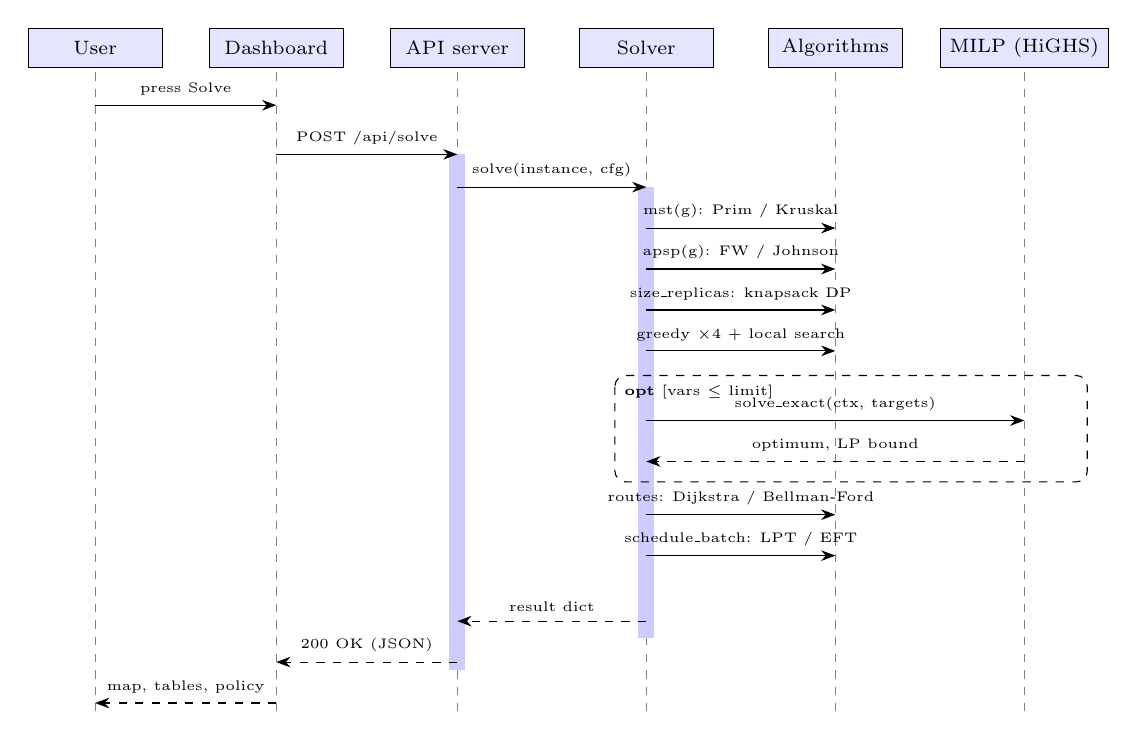
\begin{tikzpicture}[font=\scriptsize, x=1cm, y=0.52cm]
  \foreach \i/\nm in {0/User, 2.3/Dashboard, 4.6/API server, 7.0/Solver, 9.4/Algorithms, 11.8/MILP (HiGHS)}{
    \node[draw, fill=blue!10, minimum width=17mm, minimum height=5mm] at (\i,0) {\nm};
    \draw[dashed, gray] (\i,-0.6) -- (\i,-16.2);}
  \fill[blue!20] (4.5,-2.6) rectangle (4.7,-15.2);
  \fill[blue!20] (6.9,-3.4) rectangle (7.1,-14.4);
  \newcommand{\msg}[4]{\draw[-{Stealth[length=1.8mm]}] (#1,#3) -- node[above,font=\tiny]{#4} (#2,#3);}
  \newcommand{\ret}[4]{\draw[-{Stealth[length=1.8mm]}, dashed] (#1,#3) -- node[above,font=\tiny]{#4} (#2,#3);}
  \msg{0}{2.3}{-1.4}{press Solve}
  \msg{2.3}{4.6}{-2.6}{POST /api/solve}
  \msg{4.6}{7.0}{-3.4}{solve(instance, cfg)}
  \msg{7.0}{9.4}{-4.4}{mst(g): Prim / Kruskal}
  \msg{7.0}{9.4}{-5.4}{apsp(g): FW / Johnson}
  \msg{7.0}{9.4}{-6.4}{size\_replicas: knapsack DP}
  \msg{7.0}{9.4}{-7.4}{greedy $\times 4$ + local search}
  \draw[dashed,rounded corners] (6.6,-8.0) rectangle (12.6,-10.6); \node[anchor=north west,font=\tiny] at (6.6,-8.0) {\textbf{opt} [vars $\le$ limit]};
  \msg{7.0}{11.8}{-9.1}{solve\_exact(ctx, targets)}
  \ret{11.8}{7.0}{-10.1}{optimum, LP bound}
  \msg{7.0}{9.4}{-11.4}{routes: Dijkstra / Bellman-Ford}
  \msg{7.0}{9.4}{-12.4}{schedule\_batch: LPT / EFT}
  \ret{7.0}{4.6}{-14.0}{result dict}
  \ret{4.6}{2.3}{-15.0}{200 OK (JSON)}
  \ret{2.3}{0}{-16.0}{map, tables, policy}
\end{tikzpicture}
\caption{Sequence diagram of \texttt{POST /api/solve}. Dashed arrows are returns; the \textbf{opt} frame runs only when the MILP is small enough.}\label{fig:sequence}
\end{figure}

\subsection{Activity diagram of the solver}
Fig.~\ref{fig:activity} shows the decisions inside the solver. Two of them are made automatically from graph size: Prim or Kruskal for the backbone, and a dense or sparse all-pairs method. If the plan does not fit in capacity, the solver falls back to first-fit-decreasing packing before local search.

\begin{figure}[!htbp]
\centering
\scalebox{0.82}{\begin{tikzpicture}[node distance=4.5mm and 8mm, font=\scriptsize]
  \node[circle, fill=black, inner sep=2.5pt] (s) {};
  \node[act, below=of s] (a1) {Validate instance};
  \node[dec, below=of a1] (d1) {$m > n\log_2 n$?};
  \node[act, below left=5mm and 2mm of d1] (p) {Prim (heap)};
  \node[act, below right=5mm and 2mm of d1] (k) {Kruskal (union-find)};
  \node[dec, below=14mm of d1] (d2) {$m\log_2 n < n^2$?};
  \node[act, below left=5mm and 2mm of d2] (j) {Johnson / repeated\\Dijkstra};
  \node[act, below right=5mm and 2mm of d2] (f) {Floyd--Warshall\\(NumPy)};
  \node[act, below=15mm of d2] (a2) {Size replicas (knapsack DP)};
  \node[act, below=of a2] (a3) {Greedy placements};
  \node[dec, below=of a3] (d3) {Capacity\\feasible?};
  \node[act, right=12mm of d3] (ffd) {FFD repair};
  \node[act, below=of d3] (a4) {Local search};
  \node[act, below=of a4] (a5) {MILP check (if small)};
  \node[act, below=of a5] (a6) {Routes, schedule, advice};
  \node[circle, draw, inner sep=2pt, below=of a6] (e) {}; \fill (e) circle (1.6pt);
  \draw[ass] (s)--(a1); \draw[ass] (a1)--(d1);
  \draw[ass] (d1) -| node[above,pos=0.2]{yes} (p); \draw[ass] (d1) -| node[above,pos=0.2]{no} (k);
  \draw[ass] (p) |- (d2); \draw[ass] (k) |- (d2);
  \draw[ass] (d2) -| node[above,pos=0.2]{yes} (j); \draw[ass] (d2) -| node[above,pos=0.2]{no} (f);
  \draw[ass] (j) |- (a2); \draw[ass] (f) |- (a2);
  \draw[ass] (a2)--(a3); \draw[ass] (a3)--(d3);
  \draw[ass] (d3) -- node[above]{no} (ffd); \draw[ass] (ffd) |- (a4);
  \draw[ass] (d3) -- node[right]{yes} (a4);
  \draw[ass] (a4)--(a5); \draw[ass] (a5)--(a6); \draw[ass] (a6)--(e);
\end{tikzpicture}}
\caption{Activity diagram of the solver pipeline with its automatic algorithm choices.}\label{fig:activity}
\end{figure}



%======================================================================
\section{Implementation and Working Screenshots}\label{sec:impl}
All screenshots were captured from the running build at $1440\times900$ using the live Python engine; the same build also runs offline on saved results.

\textbf{Landing and Home.} The landing page introduces the project and the team (Fig.~\ref{fig:ui-home}a). Home shows a live map of India or Nigeria in which yellow cities host copies and moving dots are requests travelling their shortest path to the nearest copy, followed by four headline numbers (average latency, improvement over random, gap from the optimum, solve time), the seven-stage pipeline and the ten networks. A \emph{quick tour} link starts a 13-step guided tour.

\begin{figure}[!htbp]
\centering
\begin{subfigure}{0.49\textwidth}
\includegraphics[width=\linewidth]{figures/ui_landing.png}\caption{Landing page with the team.}\end{subfigure}\hfill
\begin{subfigure}{0.49\textwidth}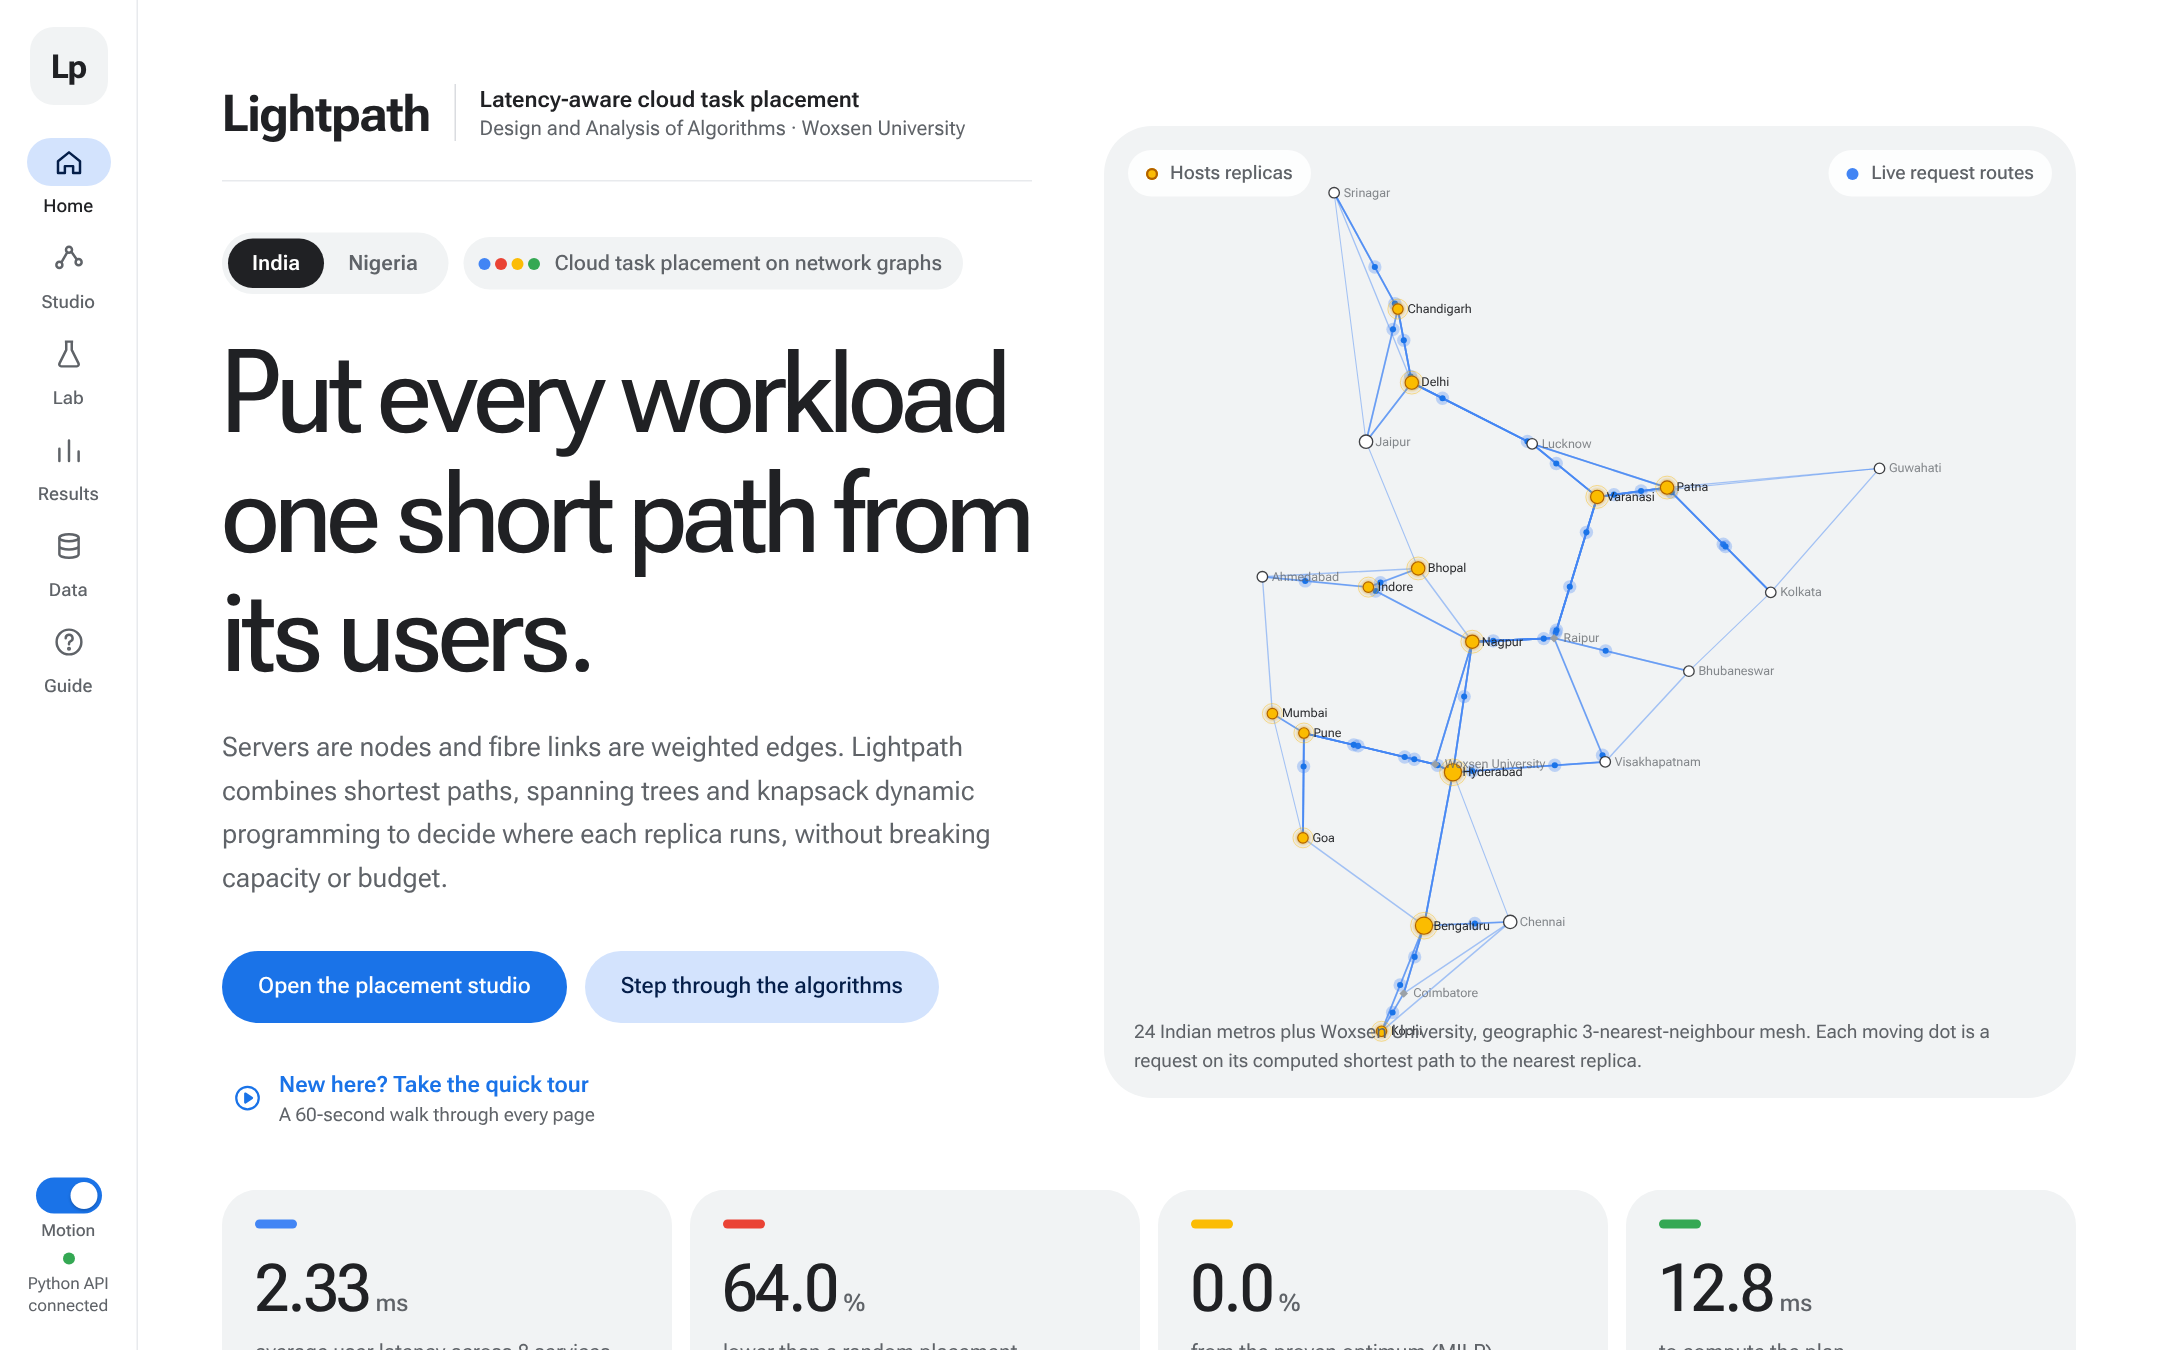
\includegraphics[width=\linewidth]{figures/ui_home.png}\caption{Home: live request map and headline numbers.}\end{subfigure}
\caption{Landing and Home pages.}\label{fig:ui-home}
\end{figure}

\textbf{Placement Studio} (Fig.~\ref{fig:ui-studio}). The user chooses a network, the VM budget, an optional server budget, the sizing method and the strategies to compare, then presses \emph{Solve placement}. The map shows where every service runs, with layers for the MST backbone, copies and routes. The right panel compares every strategy against the exact optimum and gives plain-language advice. Tabs show the route table, server load, the cost-benefit of each extra copy, replica-sync routes and the batch schedule.

\begin{figure}[!htbp]
\centering
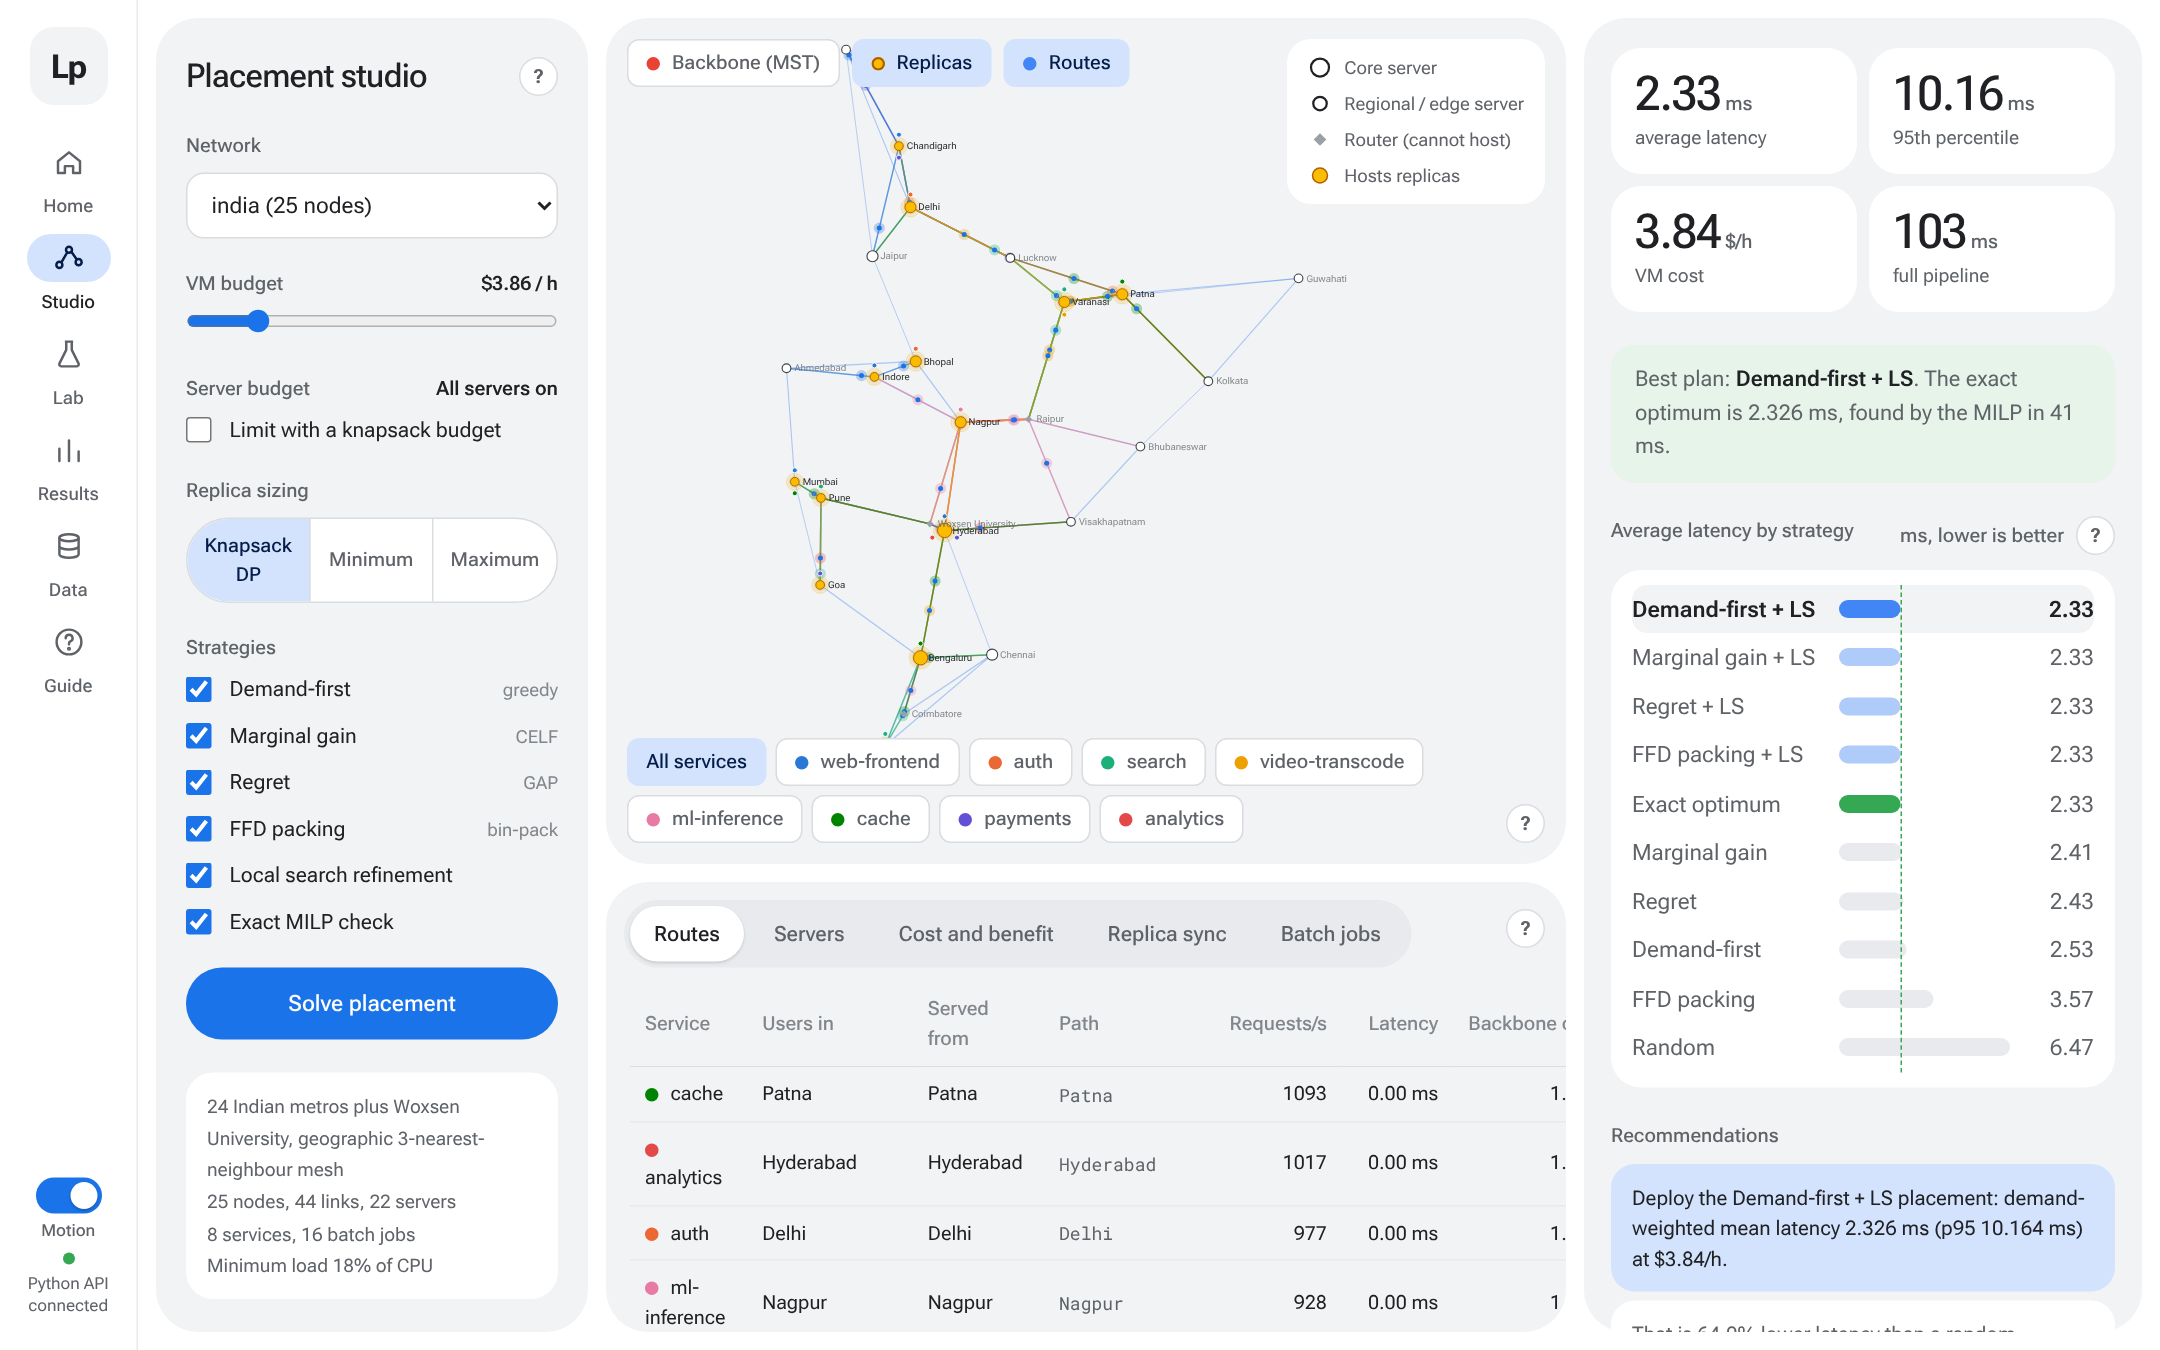
\includegraphics[width=0.8\textwidth]{figures/ui_studio.png}
\caption{Placement Studio solving the India network.}\label{fig:ui-studio}
\end{figure}

\textbf{Algorithm Lab} (Fig.~\ref{fig:ui-lab}). Any of the six graph algorithms can be replayed step by step with its pseudocode highlighted. The user picks a \textbf{start city} and a \textbf{destination} and a speed from 0.5$\times$ to 4$\times$. When the run ends, the route is drawn in blue and listed hop by hop with its delay and cost. Dijkstra and Prim stop early once the destination is final, which shows why Dijkstra suits a single trip; Bellman-Ford shows the red rebate arcs; Floyd--Warshall and Johnson show the full distance table as a heat map. \textbf{Compare two algorithms} runs two algorithms on the same trip, shows both routes side by side with a table of delay, hops, cost and work, and states which suits the trip best.

\begin{figure}[!htbp]
\centering
\begin{subfigure}{0.49\textwidth}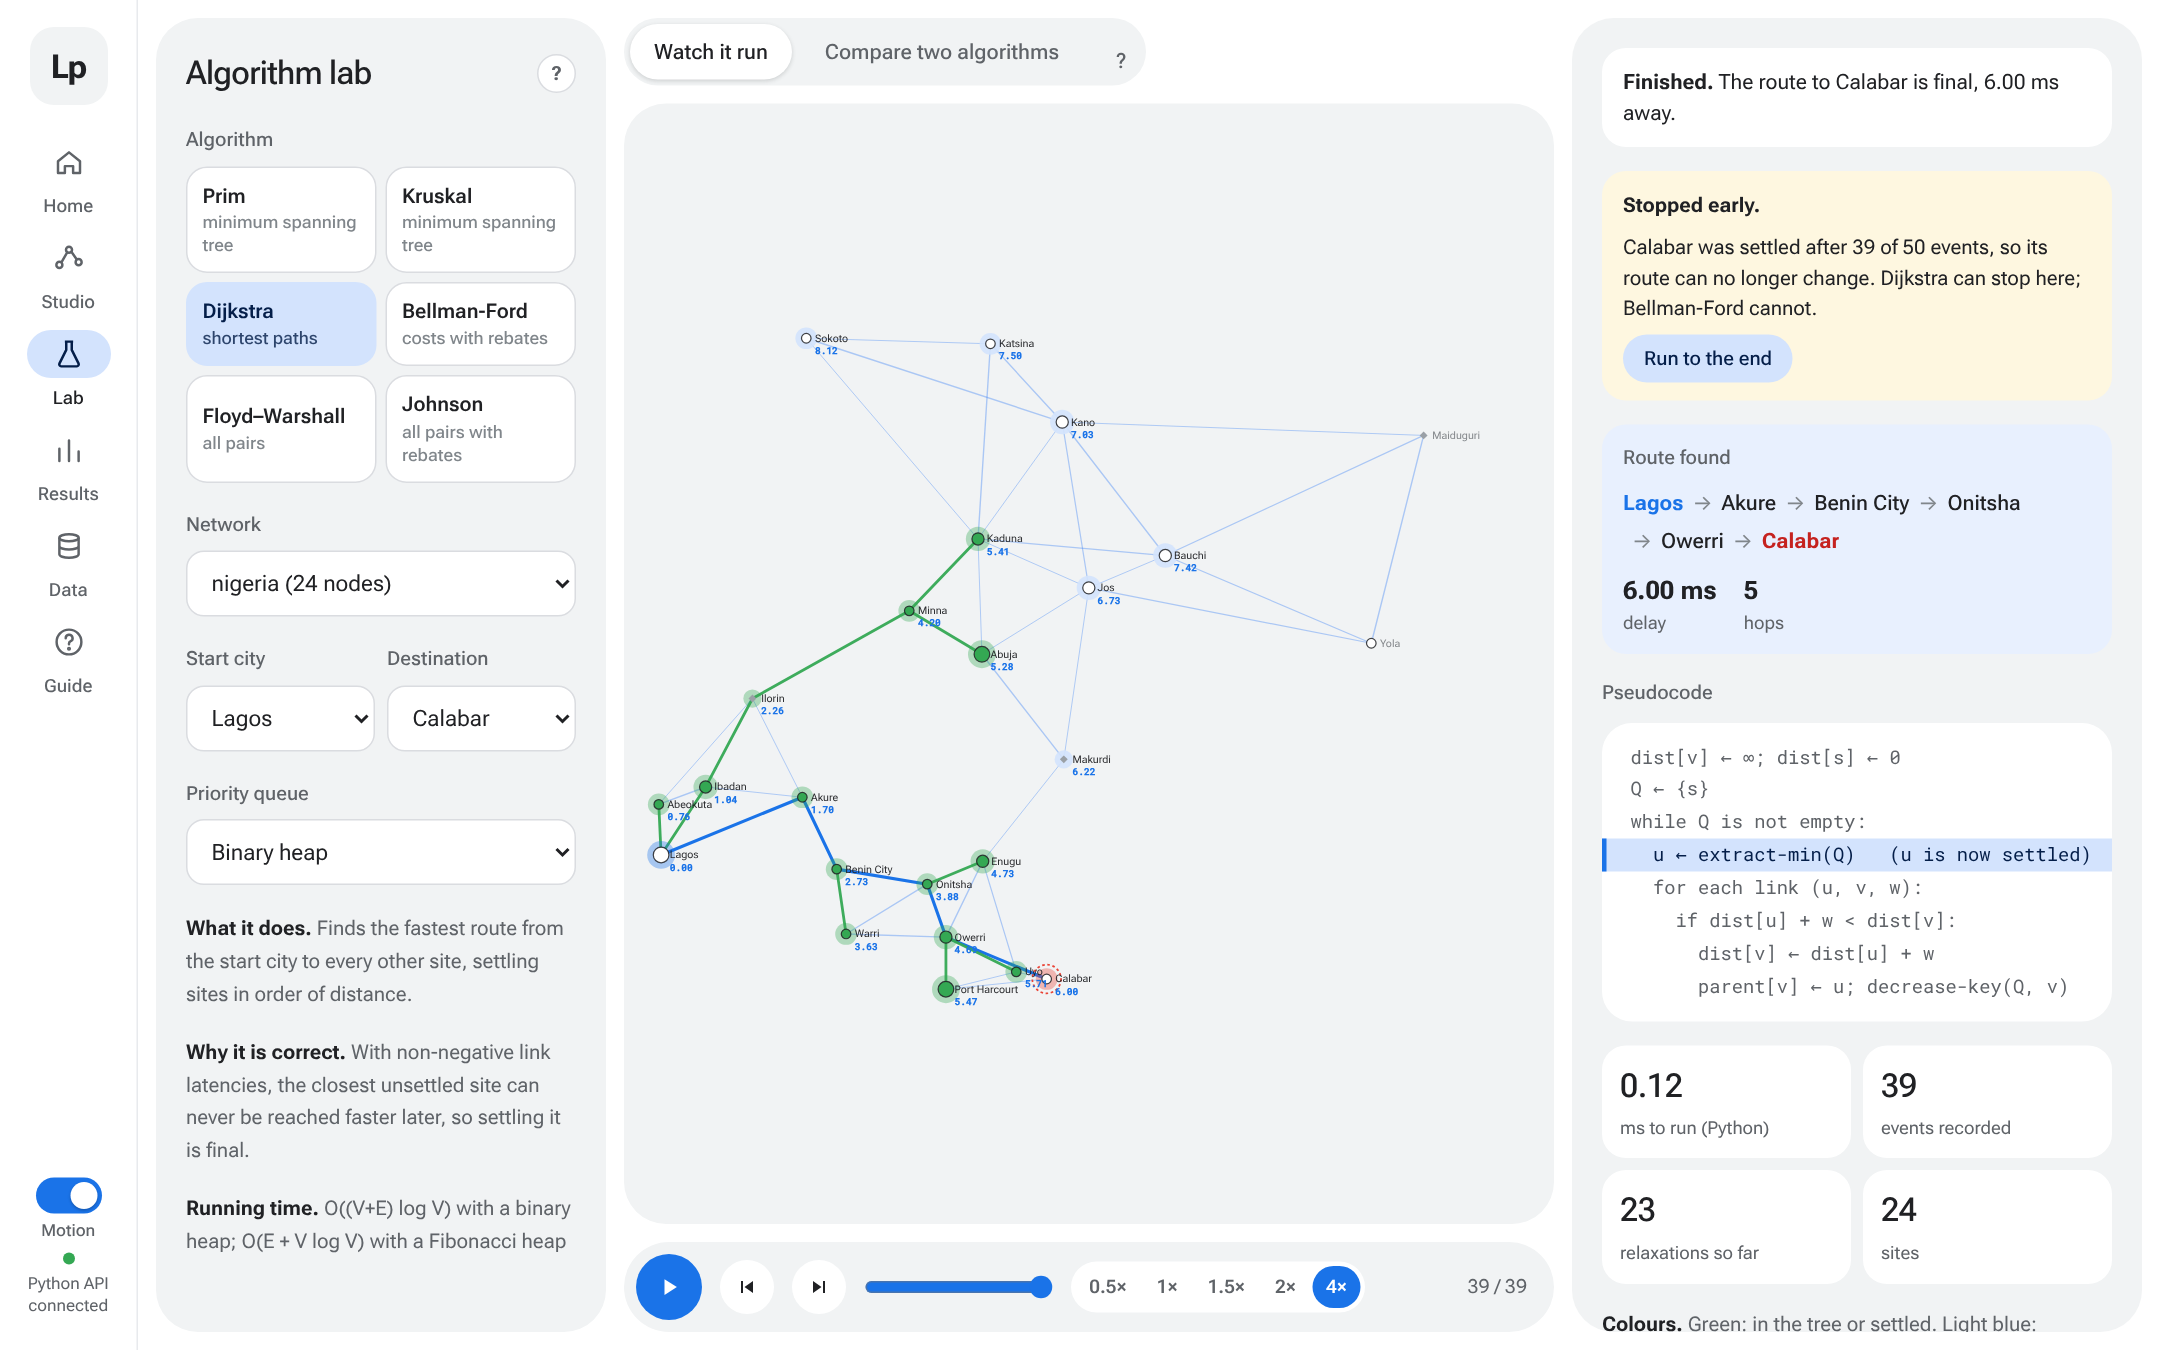
\includegraphics[width=\linewidth]{figures/ui_lab_route.png}\caption{Dijkstra from Lagos to Calabar, stopped early.}\end{subfigure}\hfill
\begin{subfigure}{0.49\textwidth}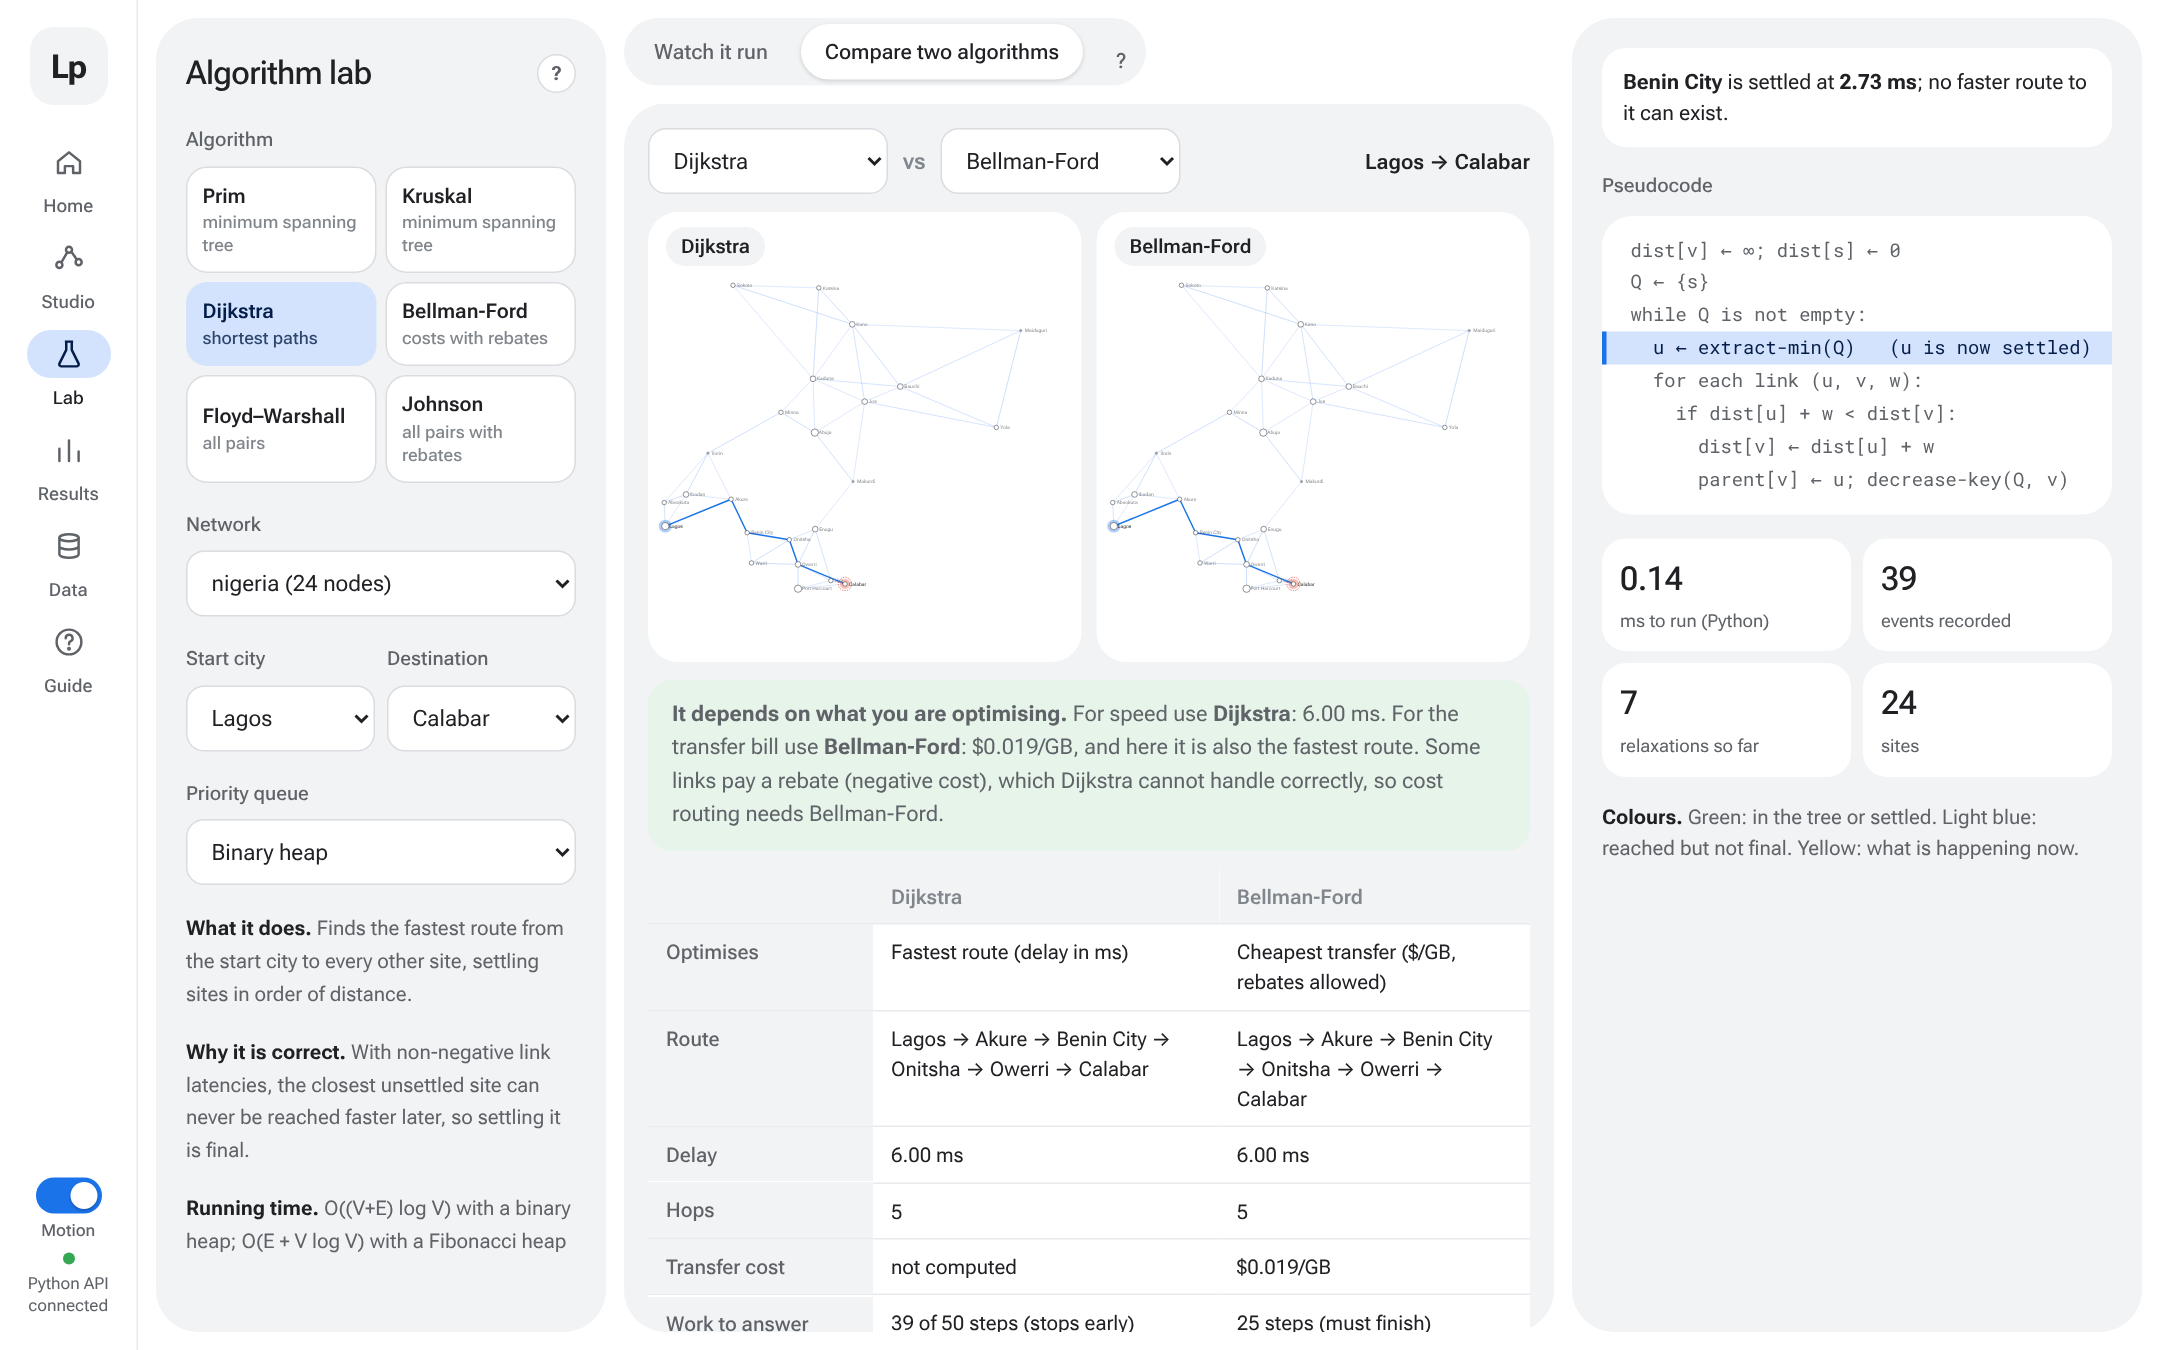
\includegraphics[width=\linewidth]{figures/ui_lab_compare.png}\caption{Comparing Dijkstra and Bellman-Ford.}\end{subfigure}
\caption{Algorithm Lab.}\label{fig:ui-lab}
\end{figure}

\textbf{Results, Data and Guide.} Results presents the eight experiments as interactive charts with one-line takeaways and CSV downloads. Data lists all ten networks with JSON, Gephi and CSV downloads and a generator for new random networks. The Guide explains every page in plain language, and every panel has a \textbf{?} help button.

\textbf{Running it.} In the project folder, \texttt{./run.sh} (macOS/Linux) or \texttt{run.bat} (Windows) installs the Python packages, builds the website and opens \url{http://localhost:8000}; \texttt{python -m pytest} runs the tests and \texttt{python experiments/run\_experiments.py} the experiments. The source code is at \url{https://github.com/namansingla-glitch/lightpath-cloud-task-placement}.

%======================================================================
\section{Complexity Analysis}\label{sec:cx}
Table~\ref{tab:cx} summarises the cost of each stage, using $V$ for sites, $E$ for links, $W$ for the budget in cents, $J$ for services, $k$ for copies per service and $S$ for servers. The dominant cost on large networks is the all-pairs latency matrix. On small networks with many services, greedy placement and local search dominate. The exact MILP is exponential in the worst case, which is why it serves only as a referee.

\begin{table}[!htbp]
\centering\small
\caption{Time complexity and guarantees by pipeline stage.}\label{tab:cx}
\begin{tabularx}{\textwidth}{@{}p{2.7cm}p{3.6cm}p{4.2cm}X@{}}
\toprule
Stage & Algorithm & Time & Guarantee\\
\midrule
Backbone & Prim (binary heap) & $O(E\log V)$ & exact (cut property)\\
 & Prim (Fibonacci heap) & $O(E + V\log V)$ & exact\\
 & Kruskal + union-find & $O(E\log E)$ & exact\\
Routing & Dijkstra & $O((V+E)\log V)$ & exact for non-negative weights\\
 & Bellman-Ford & $O(VE)$ & exact with negative edges; detects negative cycles\\
Latency matrix & Floyd--Warshall & $\Theta(V^3)$ & exact\\
 & Johnson & $O(VE + V(V+E)\log V)$ & exact with negative edges\\
Activation & 0/1 knapsack DP & $\Theta(SW)$ & optimal for the given values\\
Sizing & Multiple-choice knapsack DP & $\Theta(W\cdot\sum\text{options})$ & optimal for the given values\\
Placement & 4 greedy schedulers & polynomial, about $O(J k S V)$ & heuristic; $1-1/e$ for CELF without capacities\\
Refinement & Relocate/swap local search & polynomial per pass & local optimum; never worse than its input\\
Referee & MILP (HiGHS) & exponential worst case & proven optimum or lower bound\\
Batch & LPT, earliest finish & $O(T\log T + T S)$ & within $\tfrac43$ of optimal without transfers\\
\bottomrule
\end{tabularx}
\end{table}

%======================================================================
\section{Testing and Demonstrated Scenarios}\label{sec:test}

\subsection{Automated test suite}
Correctness is checked by 191 automated tests (Table~\ref{tab:tests}), all passing. Each algorithm is compared with an \emph{independent} reference rather than only with our own expectations: graph algorithms against NetworkX on random graphs, knapsack DPs against brute-force enumeration, and the MILP against exhaustive search on small placements.

\begin{table}[!htbp]
\centering\small
\caption{Automated test suite (191 tests, all passing).}\label{tab:tests}
\begin{tabularx}{\textwidth}{@{}l r X@{}}
\toprule
File & Tests & What is checked \\
\midrule
\texttt{test\_core.py} & 15 & Heap operations with random inputs (Hypothesis), union-find, graph construction \\
\texttt{test\_paths.py} & 66 & MST, Dijkstra, Bellman-Ford, Floyd--Warshall and Johnson against NetworkX with every heap; negative-cycle detection; no negative cycle in any transfer graph \\
\texttt{test\_optimisation.py} & 100 & Knapsack and multiple-choice knapsack against brute force; MILP against exhaustive search; greedies never exceed capacity; local search never makes a plan worse; scheduler lanes never overlap; the full pipeline on every dataset \\
\texttt{test\_api.py} & 10 & Every API endpoint, error codes and the path-traversal guard \\
\bottomrule
\end{tabularx}
\end{table}

\subsection{Scenario A: the full pipeline on India}
On the India network (25 sites, 44 links, 8 services) the solver builds a 24-link MST backbone with a total latency of 56.2\,ms, sizes the services within a \$3.86/h budget and runs all four greedy schedulers with local search. The best plan reaches an average latency of \textbf{2.326\,ms}, 64\,\% lower than a random placement, and it \emph{matches the exact MILP optimum} (gap 0.00\,\%) while taking 4.1\,ms against the MILP's 27\,ms. Mumbai, Pune, Kochi, Chandigarh and Varanasi run at 90\,\% CPU or more, so capacity there is the binding constraint.

\subsection{Scenario B: routes and negative costs}
In the Lab on the Nigeria network, Dijkstra from Lagos to Calabar finds the route Lagos $\to$ Akure $\to$ Benin City $\to$ Onitsha $\to$ Owerri $\to$ Calabar (6.00\,ms, five hops), settling the destination after 39 of 50 recorded events and stopping early. On India, the Compare view shows the same lesson for Chennai $\to$ Kochi: Dijkstra's route takes 3.93\,ms, while travelling only along Prim's spanning tree takes 5.20\,ms (1.32$\times$). Requests are therefore routed on the full network, and only the backbone is provisioned from the MST.

\noindent On transfer costs, Bellman-Ford finds the cheapest Chennai $\to$ Kochi transfer to be $-\$0.025$ per GB, a net rebate; the Compare view shows that Dijkstra cannot be trusted on these weights.

\subsection{Scenario C: capacity pressure and infeasibility}
On the \texttt{waxman-60-tight} network every server has half the normal capacity. As capacity shrinks further (Experiment E5), latency-first strategies stop finding complete plans: at $0.35\times$ capacity, demand-first, marginal gain and regret fail in every run and are reported as \emph{infeasible} rather than returned as broken plans. FFD packing still finds a valid plan at every level, so the solver uses it as a fallback. With capacity at $0.1\times$ the solver reports the shortage and every result can still be read (a dedicated test checks this).

%======================================================================
\section{Experimental Evaluation}\label{sec:exp}

\subsection{Method}
All experiments call the Python engine directly, bypassing the website. Networks come from seeded generators so that results are reproducible. Timings are medians of repeated runs on a single core in CPython 3.13, and quality results average three seeds. The full suite runs in about 80 seconds and writes CSV files and the figures below. Table~\ref{tab:data} lists the ten networks.

\begin{table}[!htbp]
\centering\small
\caption{The ten networks. Load is the CPU needed by the minimum copies divided by total capacity; best is the recommended plan's average latency.}\label{tab:data}
\begin{tabular}{@{}llrrrrrr@{}}
\toprule
Name & Source & Sites & Links & Servers & Services & Load & Best (ms)\\
\midrule
india & real coordinates + Woxsen & 25 & 44 & 22 & 8 & 18\% & 2.326\\
nigeria & real coordinates & 24 & 47 & 21 & 8 & 23\% & 1.137\\
woxsen & campus map & 23 & 29 & 13 & 8 & 17\% & 0.055\\
abilene & real topology & 11 & 14 & 10 & 6 & 42\% & 3.827\\
nsfnet & real topology & 14 & 21 & 12 & 7 & 26\% & 5.220\\
fat-tree-k4 & data centre & 36 & 48 & 16 & 6 & 18\% & 0.022\\
waxman-60 & synthetic WAN & 60 & 89 & 51 & 14 & 13\% & 5.245\\
waxman-60-tight & half capacity & 60 & 89 & 51 & 14 & 27\% & 6.686\\
er-100 & Erd\H{o}s--R\'enyi & 100 & 350 & 85 & 16 & 10\% & 5.062\\
ba-150 & Barab\'asi--Albert & 150 & 296 & 128 & 20 & 7\% & 7.594\\
\bottomrule
\end{tabular}
\end{table}

\noindent Abilene and NSFNET are real US research backbones. India (24 metros plus Woxsen University) and Nigeria (24 cities, with Lagos, Abuja and Port Harcourt as core data centres) use real city coordinates with each city linked to its three nearest neighbours. The Woxsen campus has 23 buildings laid out from the official campus map. The synthetic families let us vary size and density: Waxman geographic networks \cite{waxman1988}, Erd\H{o}s--R\'enyi random graphs, Barab\'asi--Albert hub-heavy graphs \cite{barabasi1999} and a data-centre fat-tree.

\subsection{E1: priority queues}
\begin{figure}[!htbp]
\centering
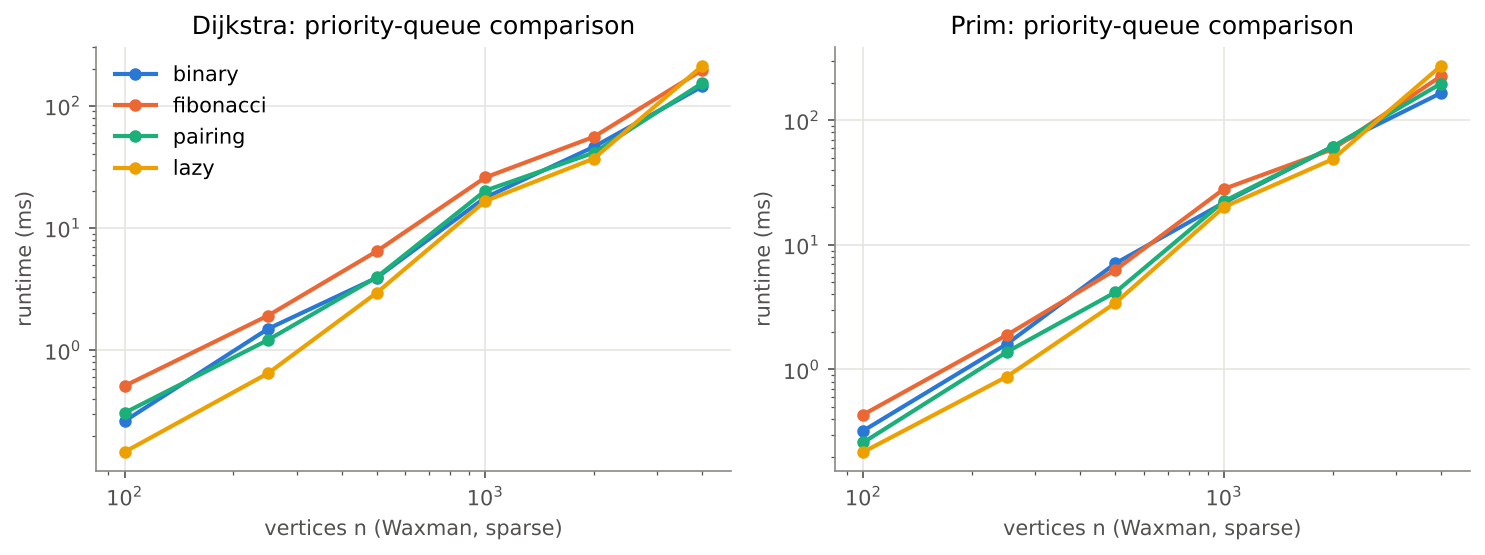
\includegraphics[width=0.64\textwidth]{figures/e1_heaps.png}
\caption{E1: Dijkstra and Prim with four priority queues on sparse graphs of up to 4000 sites.}\label{fig:e1}
\end{figure}
The Fibonacci heap has the best Big-O bound but was consistently \emph{slower} (Fig.~\ref{fig:e1}). At 1000 sites Dijkstra took 25.9\,ms with it against 17.7\,ms with the binary heap, and at 4000 sites 196\,ms against 144\,ms. Its pointer-heavy nodes and consolidation cost more in an interpreter than the decrease-key operations it saves. Python's built-in lazy heap is fastest up to 2000 sites but falls behind at 4000 as stale entries accumulate.

\subsection{E2: all-pairs shortest paths}
\begin{figure}[!htbp]
\centering
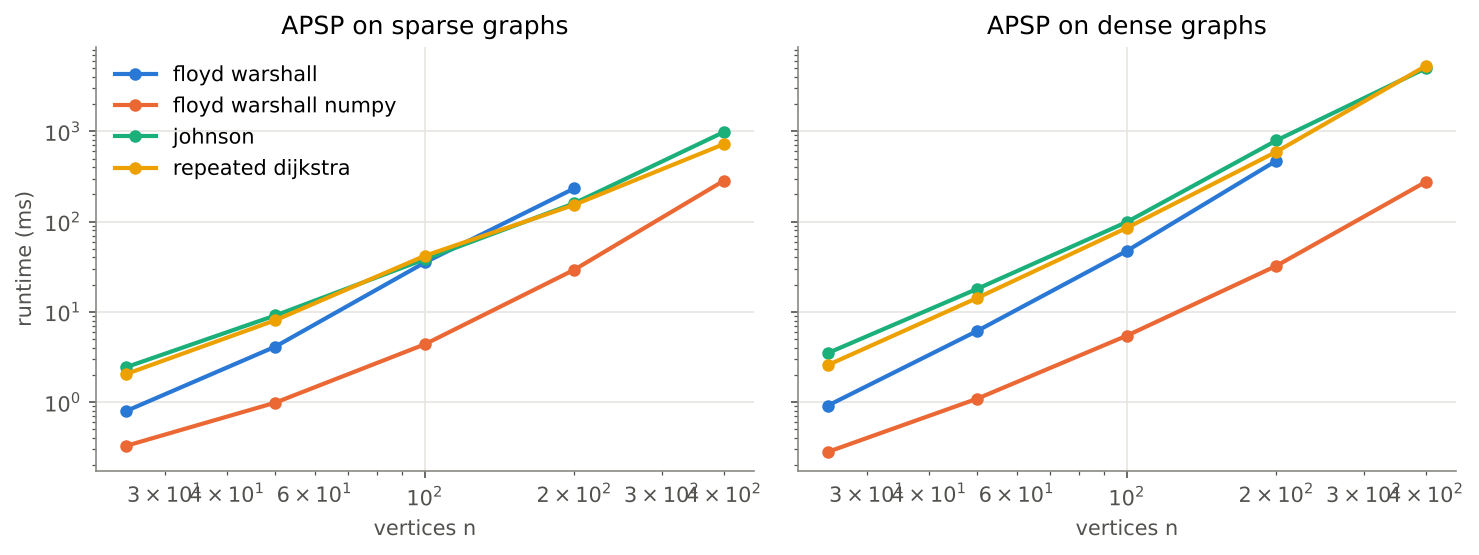
\includegraphics[width=0.64\textwidth]{figures/e2_apsp.png}
\caption{E2: all-pairs algorithms on sparse and dense graphs.}\label{fig:e2}
\end{figure}
On dense graphs (Fig.~\ref{fig:e2}) the vectorised Floyd--Warshall wins clearly: 277\,ms at 400 sites against 5015\,ms for Johnson and 5323\,ms for repeated Dijkstra. On sparse graphs repeated Dijkstra (724\,ms) beats Johnson (985\,ms), but NumPy Floyd--Warshall is still faster (285\,ms). The asymptotic rule correctly predicts that Dijkstra beats a pure-Python $V^3$ loop (234\,ms already at 200 sites), but vectorisation moves the crossover well beyond 400 sites.

\subsection{E3: spanning trees versus density}
\begin{figure}[!htbp]
\centering
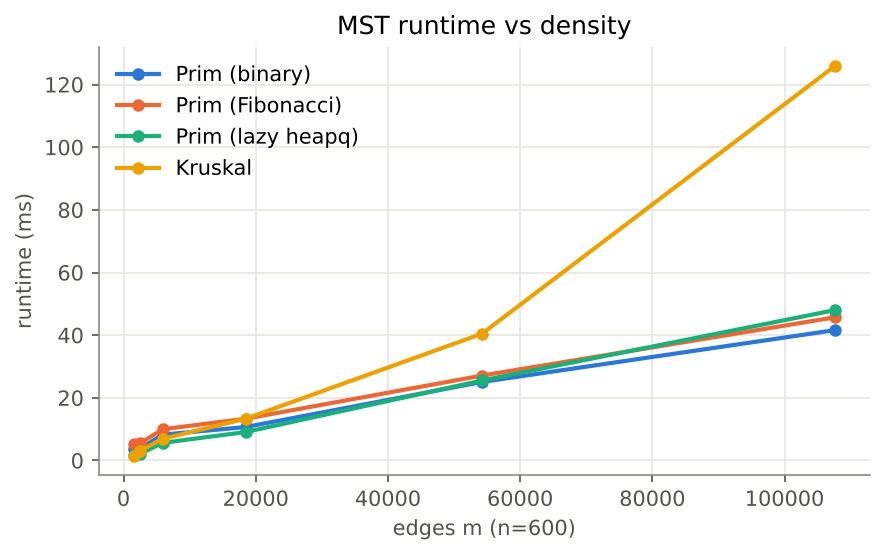
\includegraphics[width=0.55\textwidth]{figures/e3_mst.png}
\caption{E3: Prim with four heaps against Kruskal as edge density grows (600 sites).}\label{fig:e3}
\end{figure}
With 600 sites and 1.5k to 108k links (Fig.~\ref{fig:e3}), Kruskal is fastest on sparse graphs (1.5\,ms against 3.7\,ms) and slowest on dense ones (126\,ms against 42\,ms), exactly as its sort-dominated cost predicts. Every variant returned the same tree weight.

\subsection{E4: solution quality and cost versus size}
\begin{figure}[!htbp]
\centering
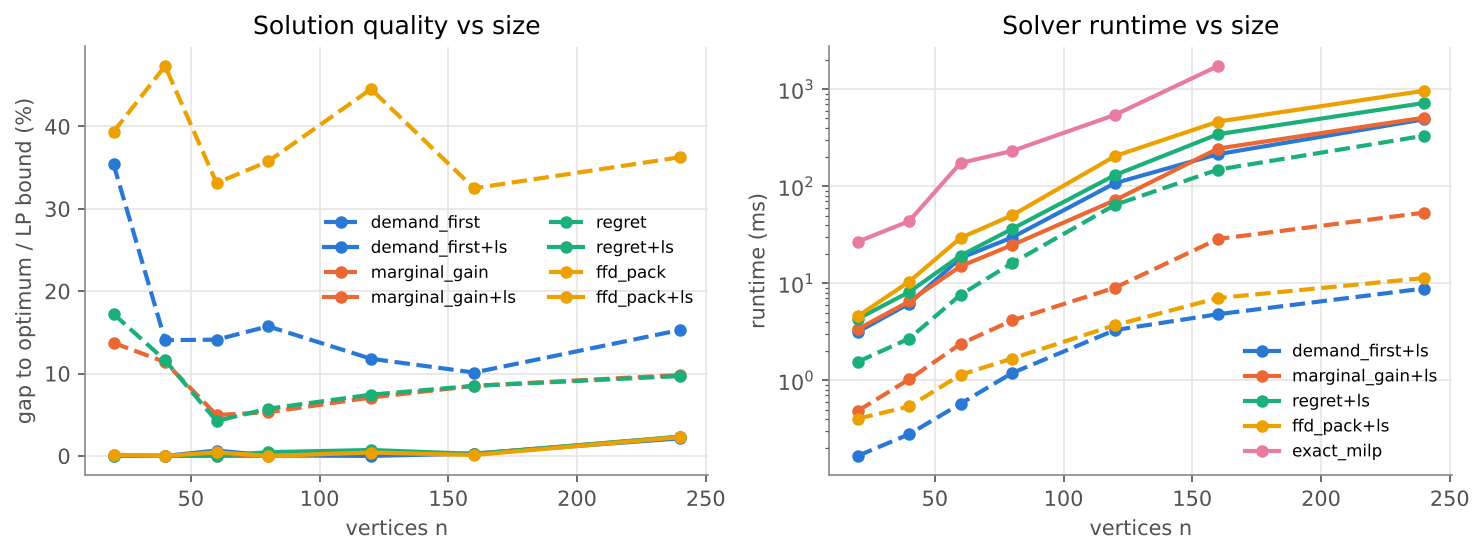
\includegraphics[width=0.64\textwidth]{figures/e4_quality_size.png}
\caption{E4: distance from the optimum (left) and run time (right) as networks grow. Dashed lines are greedy alone; solid lines include local search.}\label{fig:e4}
\end{figure}
This is the main quality experiment (Fig.~\ref{fig:e4}, Table~\ref{tab:gap}). Averaged over networks of 20 to 240 servers, greedy alone is 8.7\,\% (marginal gain), 9.2\,\% (regret), 16.7\,\% (demand-first) and 38.4\,\% (FFD) above the optimum, while a random placement is 167\,\% above. \textbf{Local search brings every method to about 0.5\,\% on average}, with a worst case of about 3\,\%. The exact MILP grows from 27\,ms at 20 servers to 1.7\,s at 160, against 4\,ms and 344\,ms for regret with local search, about five times cheaper. Greedy alone is 10 to 100 times cheaper than the MILP.

\begin{table}[!htbp]
\centering\small
\caption{E4: average distance from the MILP optimum (\%) on Waxman networks, three seeds per size.}\label{tab:gap}
\begin{tabular}{@{}lrrrrrr@{}}
\toprule
Strategy & 20 servers & 40 & 60 & 80 & 120 & 160 \\
\midrule
Random & 186.63 & 163.01 & 165.61 & 137.93 & 166.80 & 172.12 \\
FFD packing & 39.35 & 47.34 & 33.14 & 35.75 & 44.54 & 32.50 \\
Demand-first & 35.41 & 14.06 & 14.11 & 15.73 & 11.80 & 10.12 \\
Regret & 17.23 & 11.61 & 4.24 & 5.73 & 7.44 & 8.51 \\
Marginal gain & 13.73 & 11.39 & 4.97 & 5.30 & 7.09 & 8.51 \\
\midrule
FFD packing + LS & 0.14 & 0.00 & 0.44 & 0.00 & 0.41 & 0.11 \\
Demand-first + LS & 0.00 & 0.00 & 0.65 & 0.05 & 0.00 & 0.29 \\
Regret + LS & 0.00 & 0.00 & 0.00 & 0.45 & 0.72 & 0.24 \\
Marginal gain + LS & 0.14 & 0.00 & 0.00 & 0.00 & 0.52 & 0.24 \\
\bottomrule
\end{tabular}
\end{table}

\subsection{E5: capacity pressure}
\begin{figure}[!htbp]
\centering
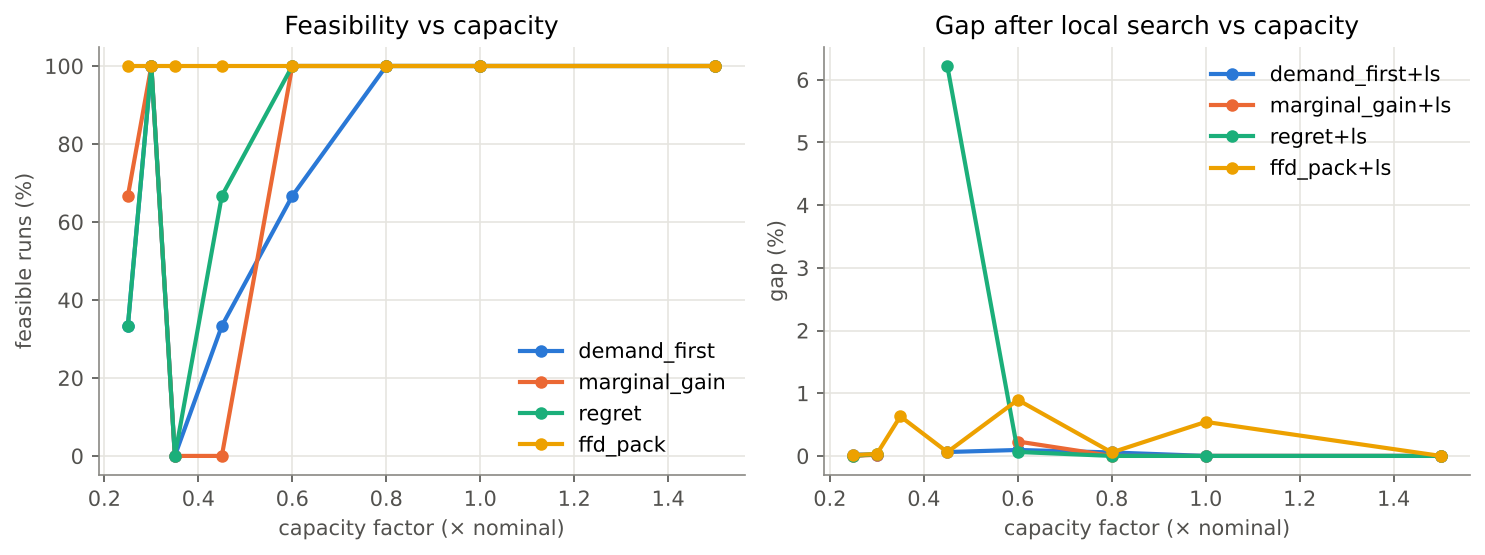
\includegraphics[width=0.64\textwidth]{figures/e5_capacity.png}
\caption{E5: share of runs with a valid plan (left) and distance from the optimum after local search (right) as server capacity shrinks.}\label{fig:e5}
\end{figure}
At normal capacity every method finds a valid plan (Fig.~\ref{fig:e5}). At $0.35\times$ capacity, the three latency-first methods fail in every run because their early choices fragment server capacity, while FFD packing remains valid at every level and local search then brings its latency close to optimal. Under tight capacity, feasibility and latency pull in different directions, and packing first is the safer strategy.

\subsection{E6, E7 and E8: density, budget and knapsack scaling}
\begin{figure}[!htbp]
\centering
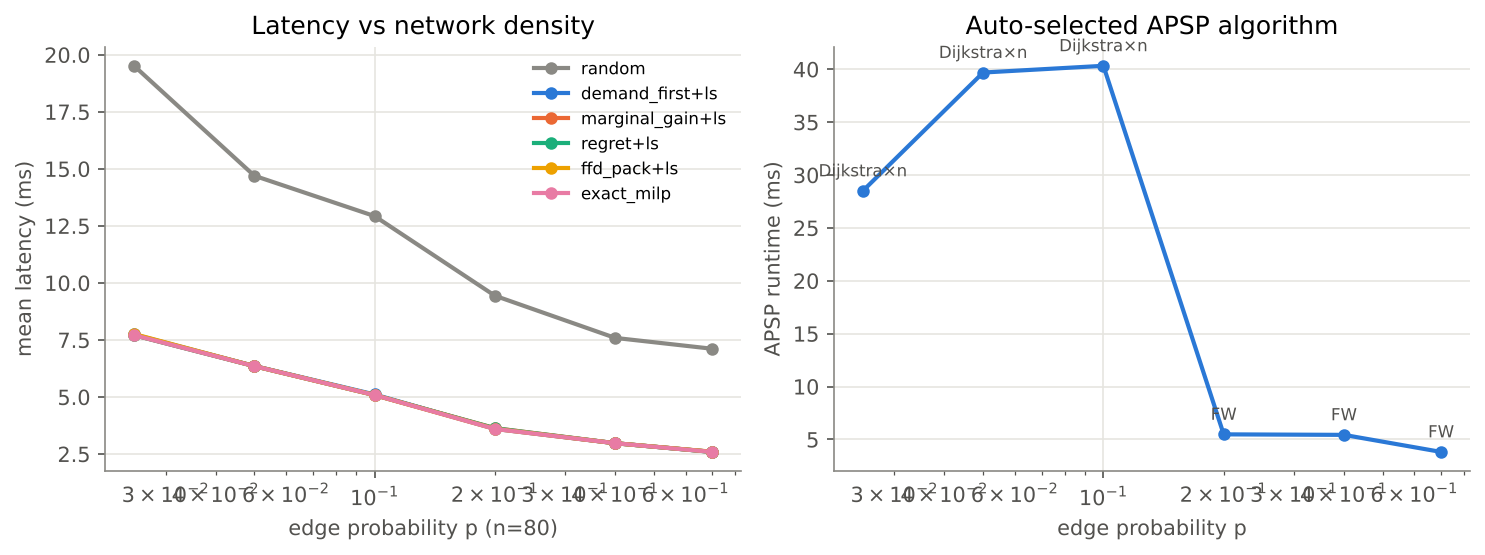
\includegraphics[width=0.62\textwidth]{figures/e6_density.png}
\caption{E6: optimal latency and heuristic gap as link density grows (80 sites).}\label{fig:e6}
\end{figure}
\textbf{E6} (Fig.~\ref{fig:e6}): raising link density from 0.025 to 0.7 cut the optimal average latency from 7.71\,ms to 2.59\,ms (67\,\%), with little extra gain beyond about 0.2. Regret plus local search matched the optimum at five of six densities. \textbf{E7}: on India, increasing the VM budget from \$2.41 to \$7.51 per hour bought 9 to 27 copies and cut latency from 4.34\,ms to 1.28\,ms (70\,\%), with diminishing returns. \textbf{E8}: knapsack run time grew linearly with table size, about 97\,ns per cell, confirming the $\Theta(nW)$ bound (Fig.~\ref{fig:e78}).

\begin{figure}[!htbp]
\centering
\begin{subfigure}{0.49\textwidth}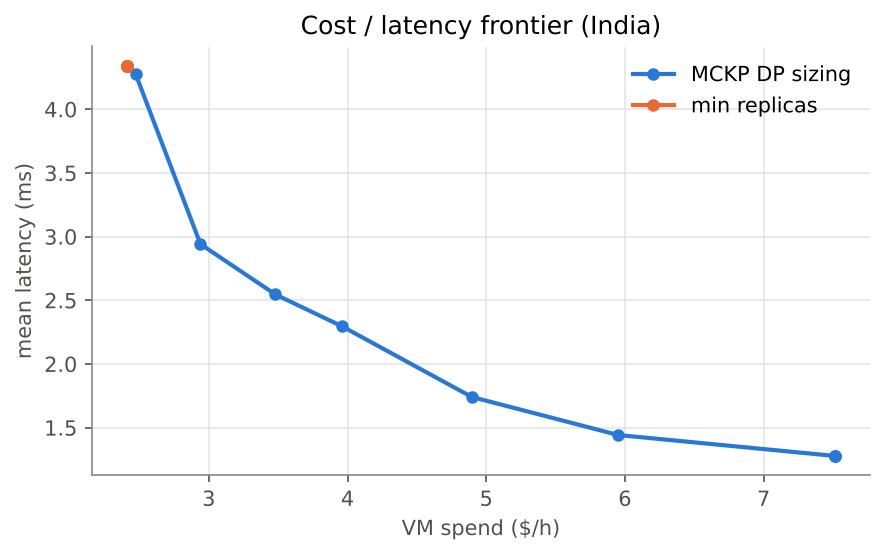
\includegraphics[width=\linewidth]{figures/e7_budget.png}\caption{E7: budget against latency (India).}\end{subfigure}\hfill
\begin{subfigure}{0.49\textwidth}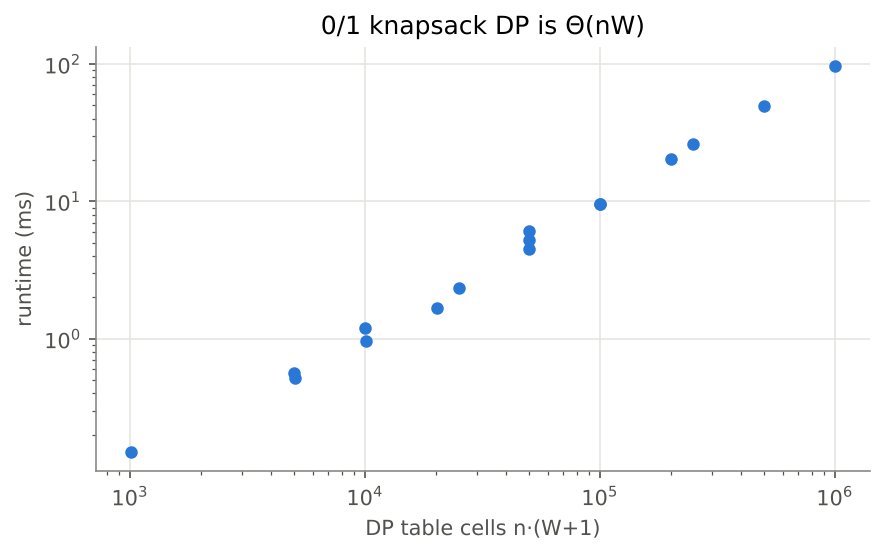
\includegraphics[width=\linewidth]{figures/e8_knapsack.png}\caption{E8: knapsack run time against table size.}\end{subfigure}
\caption{Budget frontier and knapsack scaling.}\label{fig:e78}
\end{figure}

\begin{table}[!htbp]
\centering\small
\caption{Summary of the eight experiments.}\label{tab:expsum}
\begin{tabularx}{\textwidth}{@{}l l X@{}}
\toprule
Exp. & Varied & Main finding \\
\midrule
E1 & size, heap type & Binary heap fastest at scale; Fibonacci slower in practice despite its better bound \\
E2 & size, density & NumPy Floyd--Warshall wins on dense graphs and, at these sizes, on sparse ones too \\
E3 & density & Kruskal best when sparse, Prim best when dense; identical tree weight \\
E4 & size & Greedy + local search within about 0.5\,\% of the optimum, about 5$\times$ faster than the MILP \\
E5 & capacity & Under tight capacity only FFD packing always finds a valid plan \\
E6 & density & More links cut latency by 67\,\%, with diminishing returns after density 0.2 \\
E7 & VM budget & \$2.41 $\to$ \$7.51/h cuts latency by 70\,\% (4.34 $\to$ 1.28\,ms) \\
E8 & DP table size & Linear in table size, about 97\,ns per cell \\
\bottomrule
\end{tabularx}
\end{table}

%======================================================================
\section{Case Studies and Policy Outputs}\label{sec:policy}
For every network the solver produces deployable \emph{policies}: a route table (each city, its copy, the path and latency, and the stretch if only the backbone were used), a server schedule with the VMs and utilisation of each server, a cost-benefit table giving the latency saved by each extra copy and its price, the cheapest replica-synchronisation routes, and a batch-job timetable. Table~\ref{tab:cases} and Figs.~\ref{fig:regions}--\ref{fig:woxsen} summarise the three main networks.

\begin{table}[!htbp]
\centering\small
\caption{Recommended plans. Stretch is the latency increase if requests used only the MST backbone.}\label{tab:cases}
\begin{tabular}{@{}lrrrrrl@{}}
\toprule
Network & Mean (ms) & p95 (ms) & vs.\ random & Gap from optimum & Stretch & Best next copy\\
\midrule
India & 2.326 & 10.16 & $-64.0\%$ & 0.00\,\% & 1.55$\times$ & video-transcode: $-2.45$\,ms for \$0.48/h\\
Nigeria & 1.137 & 2.88 & $-44.3\%$ & 0.09\,\% & 1.23$\times$ & analytics: $-1.23$\,ms for \$0.58/h\\
Woxsen & 0.055 & 0.21 & $-38.9\%$ & 0.00\,\% & 1.39$\times$ & dining POS: $-0.028$\,ms for \$0.06/h\\
\bottomrule
\end{tabular}
\end{table}

\begin{figure}[!htbp]
\centering
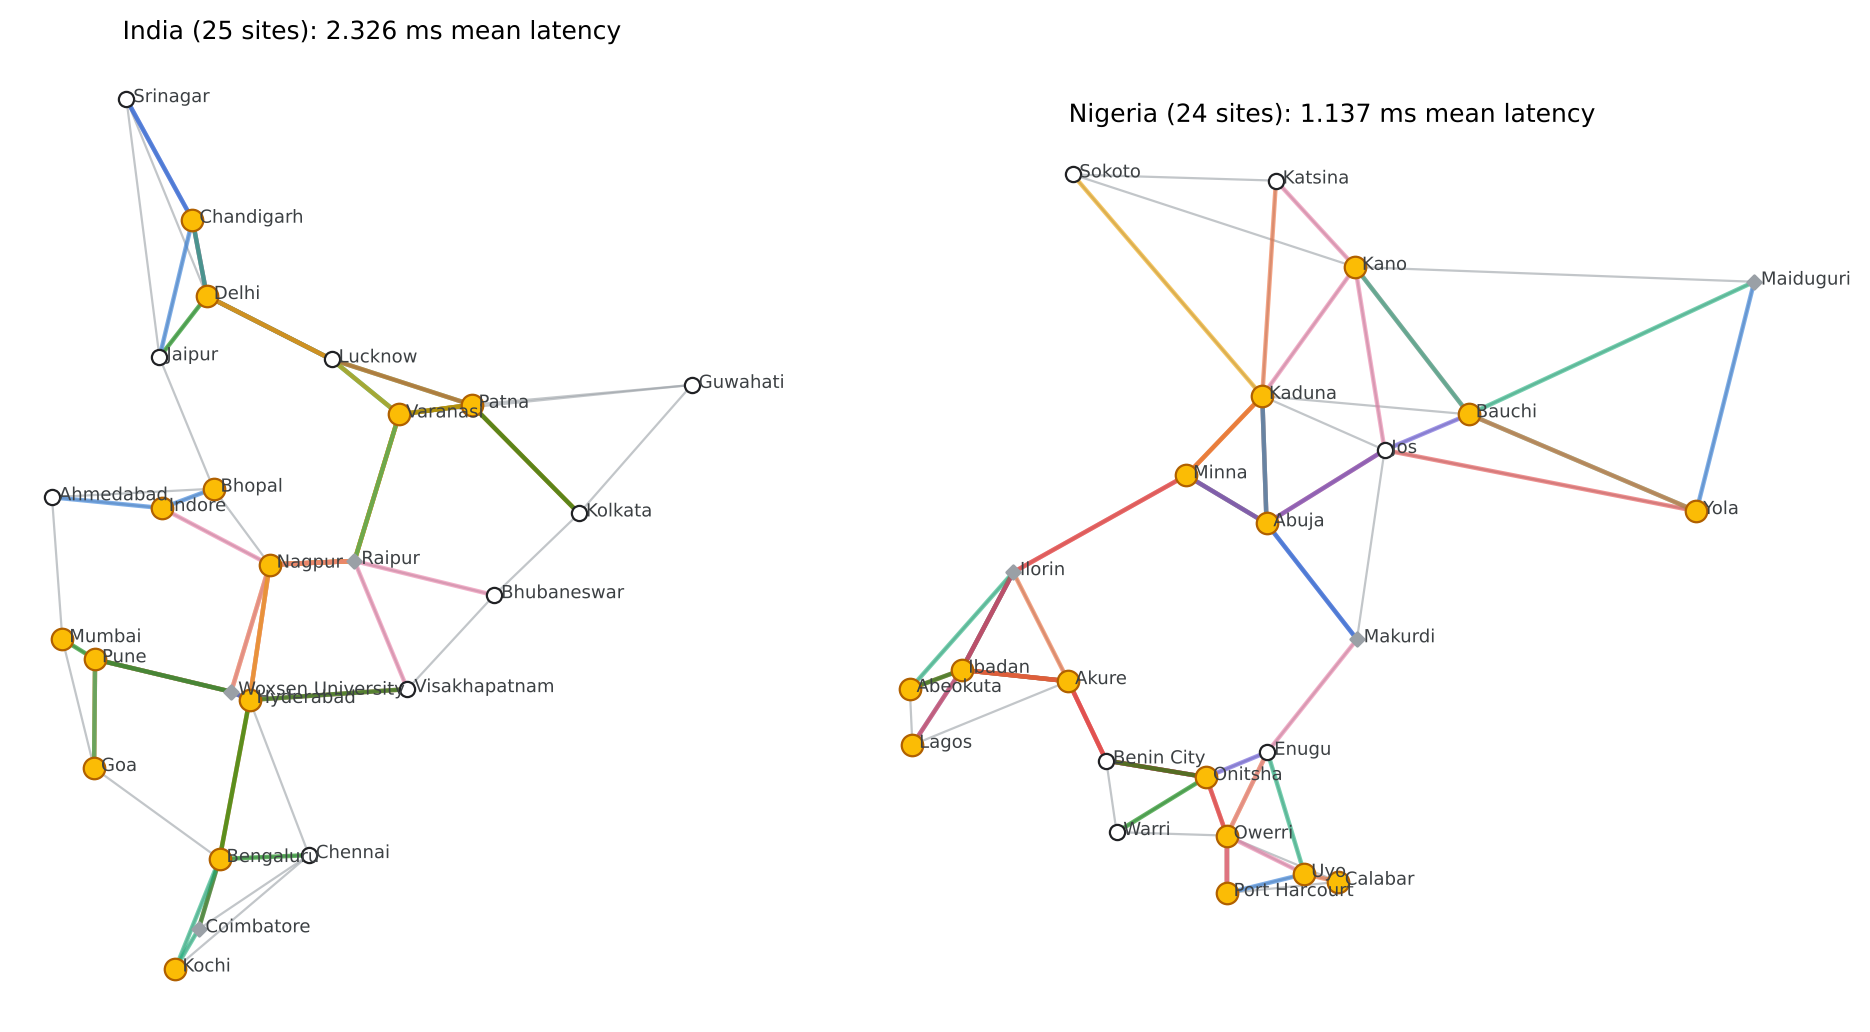
\includegraphics[width=0.8\textwidth]{figures/plans_regions.png}
\caption{Recommended placements for India and Nigeria. Yellow sites host copies; coloured lines are request routes, one colour per service.}\label{fig:regions}
\end{figure}

\begin{figure}[!htbp]
\centering
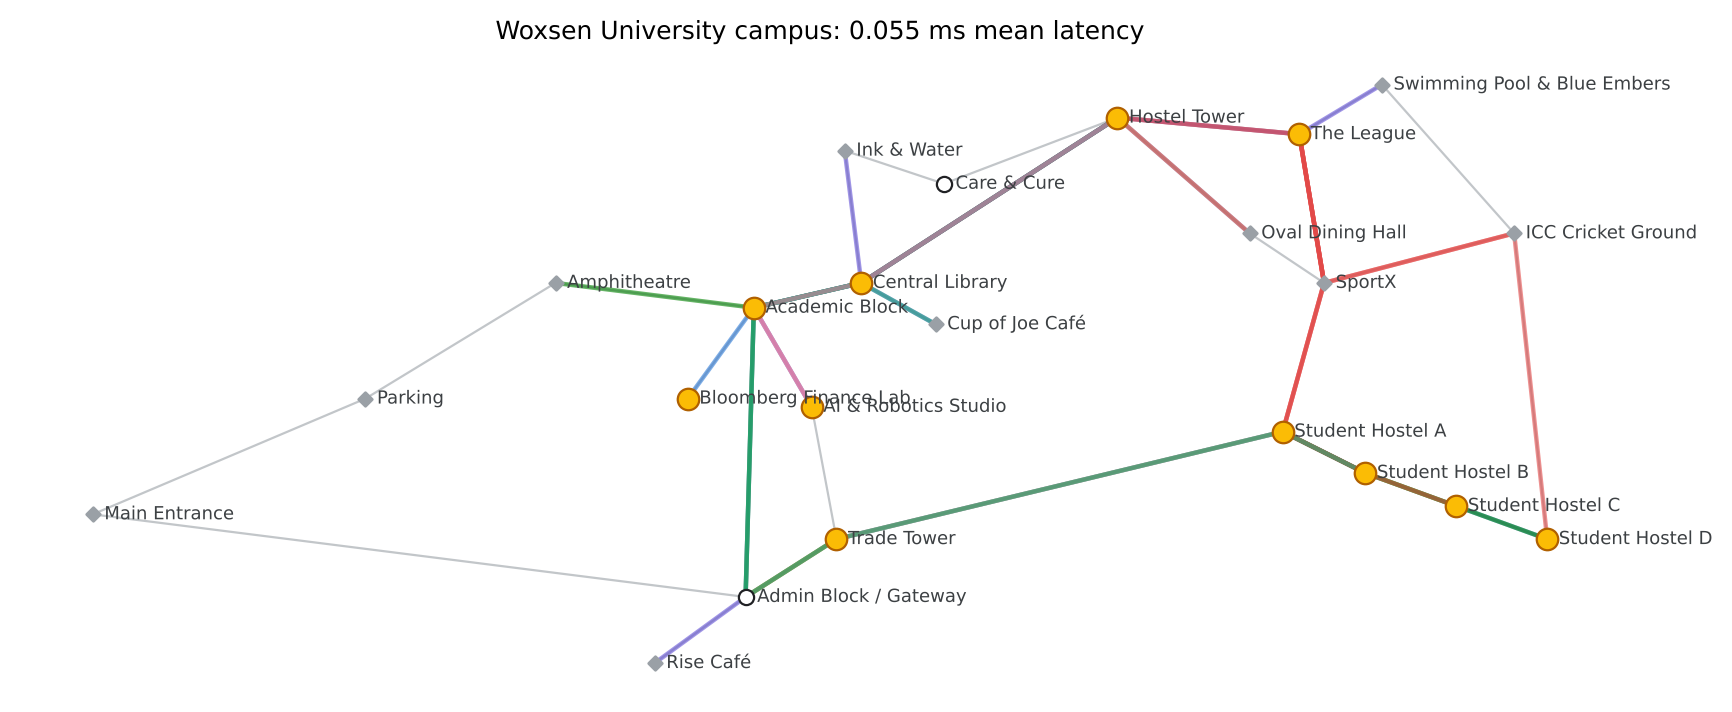
\includegraphics[width=0.72\textwidth]{figures/plan_woxsen.png}
\caption{Woxsen University campus plan. Copies cluster around the Academic Block, the hostels and The League sports arena, where demand originates.}\label{fig:woxsen}
\end{figure}

\textbf{India.} The best plan matches the MILP optimum; upgrading the saturated Mumbai, Pune, Kochi, Chandigarh and Varanasi servers is the most valuable hardware change. \textbf{Nigeria.} The MILP optimum is 1.137\,ms and marginal gain with local search is within 0.09\,\% of it. Lagos, Abuja and Port Harcourt host the core VMs while Onitsha and Owerri saturate. \textbf{Woxsen.} Every building is within 0.52\,ms. Hostel and sports traffic dominate, so the learning portal and Wi-Fi authentication replicate into Student Hostels A and D, and live streaming runs at The League.

\subsection*{Recommendations}
\begin{enumerate}[leftmargin=*]
\item \textbf{Default solver:} run all four greedy schedulers with local search and keep the best. This lands within 0.5\,\% of optimal on average, and the MILP can certify the result on smaller networks.
\item \textbf{Capacity first when load is high:} when servers are crowded, start from FFD packing, then refine for latency (E5).
\item \textbf{Spend by marginal value:} buy the next copy with the best milliseconds-per-dollar ratio from the cost-benefit table; returns diminish quickly (E7).
\item \textbf{Build the MST backbone, but route on the full network:} routing only along the tree would be 1.2--1.6$\times$ slower.
\end{enumerate}

%======================================================================
\section{Correctness Reasoning (Proof Sketches)}\label{sec:proofs}
\textbf{MST (cut property).} For any split of the sites into two groups, the cheapest crossing link belongs to some minimum spanning tree. Prim applies this to the split between tree and non-tree sites, Kruskal to the two groups a link joins, so both add only safe links and return a minimum spanning tree.
\textbf{Dijkstra.} When the closest unsettled city $u$ is taken, any other route to it must leave the settled region through a city at least as far away; with non-negative weights the rest of that route cannot shorten it, so $u$'s distance is final \cite{cormen2022}. This fails with negative weights, which is why transfer costs use Bellman-Ford.
\textbf{Bellman-Ford.} After round $i$ every route of at most $i$ links is correct; loop-free routes have at most $V-1$ links, so $V-1$ rounds suffice, and any improvement in round $V$ reveals a negative cycle.
\textbf{Knapsack DPs.} An optimal choice either skips the last item (and is optimal for the rest at the same budget) or takes it (and is optimal for the rest at the reduced budget); the table tries both, so every entry is optimal by induction.
\textbf{Local search.} Each accepted move strictly lowers latency and there are finitely many plans, so it stops, and it is never worse than its greedy start.

\begin{lemma}\label{lem:nocycle}
The transfer-cost network has negative arcs but no negative cycle.
\end{lemma}
\begin{proofsketch}
Each arc costs a positive base plus a positive per-millisecond charge plus $\varphi(u)-\varphi(v)$, the difference of two regional price levels. Around any closed loop these differences cancel, so every loop's total is positive. The same ``potential'' idea makes Johnson's reweighting correct.
\end{proofsketch}

%======================================================================
\section{Limitations and Future Work}
India and Nigeria use real city locations but synthesised links, and Woxsen's fibre plan and server sizes are modelling assumptions; real topologies such as the Internet Topology Zoo could be added. Demand is static and latency ignores queueing at busy servers, so time-varying re-placement and queueing models (for example M/M/$c$) are natural next steps. Server activation optimises an estimated value per server rather than the joint problem. Timings reflect CPython; a compiled core would extend the exact referee to larger networks.

%======================================================================
\section{Conclusion}
Lightpath shows how classical algorithm design fits a practical systems problem. Exact algorithms (Prim, Kruskal, Dijkstra, Bellman-Ford, Floyd--Warshall and Johnson) and two knapsack dynamic programs handle the tractable parts. Greedy schedulers with local search handle the NP-hard placement, and an exact solver confirms that they land within about 0.5\,\% of the optimum on average while running about five times faster. The experiments show where Big-O and measured speed agree and where they do not, and the same pipeline produces deployable plans for India, Nigeria and the Woxsen campus.


\clearpage
\renewcommand{\refname}{References}
\begin{thebibliography}{99}\footnotesize\linespread{1.0}\selectfont
\setlength{\itemsep}{2pt}
\bibitem{kariv1979} O. Kariv and S. L. Hakimi, ``An algorithmic approach to network location problems. II: The $p$-medians,'' \emph{SIAM Journal on Applied Mathematics}, vol. 37, no. 3, pp. 539--560, 1979.
\bibitem{fredman1987} M. L. Fredman and R. E. Tarjan, ``Fibonacci heaps and their uses in improved network optimization algorithms,'' \emph{Journal of the ACM}, vol. 34, no. 3, pp. 596--615, Jul. 1987.
\bibitem{tarjan1975} R. E. Tarjan, ``Efficiency of a good but not linear set union algorithm,'' \emph{Journal of the ACM}, vol. 22, no. 2, pp. 215--225, Apr. 1975.
\bibitem{prim1957} R. C. Prim, ``Shortest connection networks and some generalizations,'' \emph{Bell System Technical Journal}, vol. 36, no. 6, pp. 1389--1401, Nov. 1957.
\bibitem{kruskal1956} J. B. Kruskal, ``On the shortest spanning subtree of a graph and the traveling salesman problem,'' \emph{Proceedings of the American Mathematical Society}, vol. 7, no. 1, pp. 48--50, 1956.
\bibitem{dijkstra1959} E. W. Dijkstra, ``A note on two problems in connexion with graphs,'' \emph{Numerische Mathematik}, vol. 1, pp. 269--271, 1959.
\bibitem{bellman1958} R. Bellman, ``On a routing problem,'' \emph{Quarterly of Applied Mathematics}, vol. 16, no. 1, pp. 87--90, 1958.
\bibitem{floyd1962} R. W. Floyd, ``Algorithm 97: Shortest path,'' \emph{Communications of the ACM}, vol. 5, no. 6, p. 345, Jun. 1962.
\bibitem{johnson1977} D. B. Johnson, ``Efficient algorithms for shortest paths in sparse networks,'' \emph{Journal of the ACM}, vol. 24, no. 1, pp. 1--13, Jan. 1977.
\bibitem{nemhauser1978} G. L. Nemhauser, L. A. Wolsey, and M. L. Fisher, ``An analysis of approximations for maximizing submodular set functions---I,'' \emph{Mathematical Programming}, vol. 14, no. 1, pp. 265--294, 1978.
\bibitem{huangfu2018} Q. Huangfu and J. A. J. Hall, ``Parallelizing the dual revised simplex method,'' \emph{Mathematical Programming Computation}, vol. 10, no. 1, pp. 119--142, 2018.
\bibitem{waxman1988} B. M. Waxman, ``Routing of multipoint connections,'' \emph{IEEE Journal on Selected Areas in Communications}, vol. 6, no. 9, pp. 1617--1622, Dec. 1988.
\bibitem{barabasi1999} A.-L. Barab\'asi and R. Albert, ``Emergence of scaling in random networks,'' \emph{Science}, vol. 286, no. 5439, pp. 509--512, Oct. 1999.
\bibitem{cormen2022} T. H. Cormen, C. E. Leiserson, R. L. Rivest, and C. Stein, \emph{Introduction to Algorithms}, 4th ed. Cambridge, MA, USA: MIT Press, 2022.
\end{thebibliography}

\end{document}
